\documentclass[10pt]{article}
\usepackage[T1]{fontenc}
\usepackage[utf8]{inputenc}
\usepackage[margin=0.62in]{geometry}
\usepackage{amsmath,amssymb}
\usepackage{array,longtable}
\usepackage{graphicx,multicol}
\usepackage{xcolor}
\usepackage{hyperref}
\usepackage{tikz}
\usetikzlibrary{positioning,arrows.meta,calc}
\hypersetup{colorlinks=true,linkcolor=blue!50!black,urlcolor=blue!55!black}
\setlength{\parindent}{0pt}
\setlength{\parskip}{0.45em}
\setlength{\LTpre}{0.2em}
\setlength{\LTpost}{0.6em}
\sloppy
\newcommand{\module}[1]{\texttt{#1}}
\newcommand{\pc}{p_{\mathrm{c}}}
\newcommand{\pt}{\widetilde p}
\newcommand{\prob}{\mathbb P}
\begin{document}

\begin{center}
{\LARGE Sharpness Lean Formalization Report}\\[0.35em]
{\large Natural-language theorem inventory and dependency graph}\\[0.35em]
\small Generated from local Lean sources on 2026-06-25 01:31.
\end{center}
\section*{Proof Completion Check}

\begin{itemize}
\item \module{lake env lean Sharpness/Main.lean}: passed.
\item \module{lake build}: passed. The emitted messages were style/header linter warnings, not proof errors.
\item A source scan over all Lean files found no \module{sorry}, \module{axiom}, \module{constant}, \module{unsafe}, \module{admit}, or global \module{set\_option autoImplicit true}.
\item \module{\#print axioms Sharpness.sharpness\_zd} returned exactly \(\{\mathrm{propext},\mathrm{Classical.choice},\mathrm{Quot.sound}\}\). In particular, no \module{sorryAx} appears.
\end{itemize}

The report covers 19 Sharpness modules, 85 definitions/structures/abbreviations, and 283 theorems/lemmas. It includes 166 private supporting declarations.
\section*{Final Theorem}

The Lean theorem \module{Sharpness.sharpness\_zd} proves the following sharpness statement for nearest-neighbor Bernoulli bond percolation on \(Z^d\).

For every \(d\ge 2\):
\[
\forall p,\quad 0\le p<\pc(d)
\Longrightarrow
\exists c>0,\ \forall n\in\mathbb N,\ 
\prob_p(0\leftrightarrow\partial\Lambda_n)\le e^{-cn},
\]
and
\[
\forall p,\quad \pc(d)<p<1
\Longrightarrow
\theta_d(p)\ge
\frac{p-\pc(d)}{p(1-\pc(d))}.
\]
In Lean, \(\prob_p(0\leftrightarrow\partial\Lambda_n)\) is \module{boxExitProb d p n}, \(\theta_d(p)\) is \module{theta d p}, and \(\pc(d)\) is \module{pCrit d}.

\section*{Core Theorems in Mathematical Language}
\begin{longtable}{>{\raggedright\arraybackslash}p{0.25\textwidth} >{\raggedright\arraybackslash}p{0.68\textwidth}}
\textbf{Name} & \textbf{Natural-language mathematical statement} \\
\hline
\endfirsthead
\textbf{Name} & \textbf{Natural-language mathematical statement} \\
\hline
\endhead
{\footnotesize\ttfamily russo\_\allowbreak{}closed\_\allowbreak{}pivotal} & Russo's formula for finite local increasing events: the derivative of the event probability equals the closed-pivotal probability sum divided by 1-p. \\[0.45em]
{\footnotesize\ttfamily differential\_\allowbreak{}inequality} & For a finite volume Lambda containing the origin, the derivative of the exit probability is bounded below by phiMinIn(p,Lambda)/(p(1-p)) times one minus the exit probability. \\[0.45em]
{\footnotesize\ttfamily ode\_\allowbreak{}log\_\allowbreak{}comparison} & A real-valued function satisfying the differential lower bound f'(t) >= (1 - f(t))/(t(1 - t)) obeys the corresponding logarithmic comparison inequality between q and p. \\[0.45em]
{\footnotesize\ttfamily supercritical\_\allowbreak{}lower\_\allowbreak{}bound\_\allowbreak{}above\_\allowbreak{}pTilde} & Above the finite-set critical point pTilde and below 1, theta is bounded below by the explicit mean-field expression (p - pTilde)/(p(1 - pTilde)). \\[0.45em]
{\footnotesize\ttfamily boundary\_\allowbreak{}inequality} & The probability of connecting from u to B inside T is bounded by a sum over the oriented boundary of S, with one factor for reaching the boundary point in S, one factor p for the boundary bond, and one factor for connecting onward inside T. \\[0.45em]
{\footnotesize\ttfamily exponential\_\allowbreak{}decay\_\allowbreak{}below\_\allowbreak{}pTilde} & Below the finite-set critical point pTilde, finite box exit probabilities decay exponentially. \\[0.45em]
{\footnotesize\ttfamily pTilde\_\allowbreak{}eq\_\allowbreak{}pCrit} & In positive dimension, the finite-set critical point equals the theta-critical point. \\[0.45em]
{\footnotesize\ttfamily sharpness\_\allowbreak{}zd} & For every dimension d >= 2, subcritical finite box exit probabilities decay exponentially below p\_c(d), and above p\_c(d) the density theta\_d(p) is bounded below by (p - p\_c(d))/(p(1 - p\_c(d))). \\[0.45em]
\end{longtable}

\section*{Module Dependency Graph}

\begin{center}
\resizebox{\textwidth}{!}{%
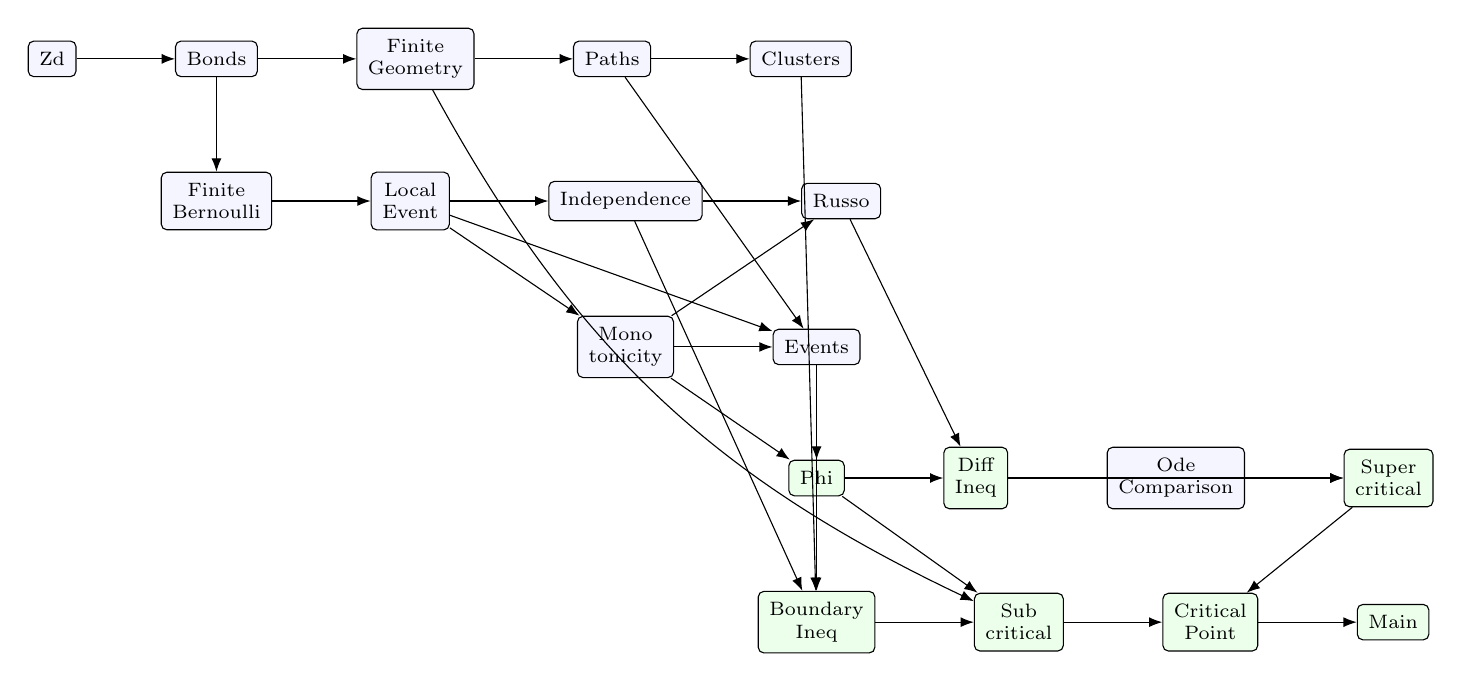
\begin{tikzpicture}[
  node distance=1.2cm and 1.25cm,
  mod/.style={draw, rounded corners=2pt, align=center, font=\scriptsize, fill=blue!4, inner sep=4pt},
  emph/.style={draw, rounded corners=2pt, align=center, font=\scriptsize, fill=green!8, inner sep=4pt},
  arr/.style={-Latex, thin}
]
\node[mod] (Zd) {Zd};
\node[mod, right=of Zd] (Bonds) {Bonds};
\node[mod, right=of Bonds] (FG) {Finite\\Geometry};
\node[mod, right=of FG] (Paths) {Paths};
\node[mod, right=of Paths] (Clusters) {Clusters};
\node[mod, below=of Bonds] (FB) {Finite\\Bernoulli};
\node[mod, right=of FB] (Local) {Local\\Event};
\node[mod, right=of Local] (Indep) {Independence};
\node[mod, below=of Indep] (Mono) {Mono\\tonicity};
\node[mod, right=of Indep] (Russo) {Russo};
\node[mod, right=of Mono] (Events) {Events};
\node[emph, below=of Events] (Phi) {Phi};
\node[emph, right=of Phi] (Diff) {Diff\\Ineq};
\node[mod, right=of Diff] (Ode) {Ode\\Comparison};
\node[emph, right=of Ode] (Super) {Super\\critical};
\node[emph, below=of Phi] (Boundary) {Boundary\\Ineq};
\node[emph, right=of Boundary] (Sub) {Sub\\critical};
\node[emph, right=of Sub] (Crit) {Critical\\Point};
\node[emph, right=of Crit] (Main) {Main};
\draw[arr] (Zd) -- (Bonds);
\draw[arr] (Bonds) -- (FG);
\draw[arr] (FG) -- (Paths);
\draw[arr] (Paths) -- (Clusters);
\draw[arr] (Bonds) -- (FB);
\draw[arr] (FB) -- (Local);
\draw[arr] (Local) -- (Indep);
\draw[arr] (Local) -- (Mono);
\draw[arr] (Indep) -- (Russo);
\draw[arr] (Mono) -- (Russo);
\draw[arr] (Local) -- (Events);
\draw[arr] (Mono) -- (Events);
\draw[arr] (Paths) -- (Events);
\draw[arr] (Events) -- (Phi);
\draw[arr] (Mono) -- (Phi);
\draw[arr] (Phi) -- (Diff);
\draw[arr] (Russo) -- (Diff);
\draw[arr] (Diff) -- (Super);
\draw[arr] (Ode) -- (Super);
\draw[arr] (Clusters) -- (Boundary);
\draw[arr] (Events) -- (Boundary);
\draw[arr] (Indep) -- (Boundary);
\draw[arr] (Boundary) -- (Sub);
\draw[arr] (FG) to[bend right=18] (Sub);
\draw[arr] (Phi) -- (Sub);
\draw[arr] (Sub) -- (Crit);
\draw[arr] (Super) -- (Crit);
\draw[arr] (Crit) -- (Main);
\end{tikzpicture}}
\end{center}

\subsection*{Actual Import Edges}
\begin{multicols}{2}
\begin{itemize}
\item \module{Sharpness.Zd} \(\to\) \module{Sharpness.Bonds}
\item \module{Sharpness.Bonds} \(\to\) \module{Sharpness.FiniteGeometry}
\item \module{Sharpness.FiniteGeometry} \(\to\) \module{Sharpness.Paths}
\item \module{Sharpness.LocalEvent} \(\to\) \module{Sharpness.Clusters}
\item \module{Sharpness.Paths} \(\to\) \module{Sharpness.Clusters}
\item \module{Sharpness.Bonds} \(\to\) \module{Sharpness.FiniteBernoulli}
\item \module{Sharpness.FiniteBernoulli} \(\to\) \module{Sharpness.LocalEvent}
\item \module{Sharpness.LocalEvent} \(\to\) \module{Sharpness.Independence}
\item \module{Sharpness.LocalEvent} \(\to\) \module{Sharpness.Monotonicity}
\item \module{Sharpness.Independence} \(\to\) \module{Sharpness.Russo}
\item \module{Sharpness.Monotonicity} \(\to\) \module{Sharpness.Russo}
\item \module{Sharpness.LocalEvent} \(\to\) \module{Sharpness.Events}
\item \module{Sharpness.Monotonicity} \(\to\) \module{Sharpness.Events}
\item \module{Sharpness.Paths} \(\to\) \module{Sharpness.Events}
\item \module{Sharpness.Events} \(\to\) \module{Sharpness.Phi}
\item \module{Sharpness.Monotonicity} \(\to\) \module{Sharpness.Phi}
\item \module{Sharpness.Phi} \(\to\) \module{Sharpness.DiffIneq}
\item \module{Sharpness.Russo} \(\to\) \module{Sharpness.DiffIneq}
\item \module{Sharpness.DiffIneq} \(\to\) \module{Sharpness.Supercritical}
\item \module{Sharpness.OdeComparison} \(\to\) \module{Sharpness.Supercritical}
\item \module{Sharpness.Clusters} \(\to\) \module{Sharpness.BoundaryIneq}
\item \module{Sharpness.Events} \(\to\) \module{Sharpness.BoundaryIneq}
\item \module{Sharpness.Independence} \(\to\) \module{Sharpness.BoundaryIneq}
\item \module{Sharpness.BoundaryIneq} \(\to\) \module{Sharpness.Subcritical}
\item \module{Sharpness.FiniteGeometry} \(\to\) \module{Sharpness.Subcritical}
\item \module{Sharpness.Phi} \(\to\) \module{Sharpness.Subcritical}
\item \module{Sharpness.Subcritical} \(\to\) \module{Sharpness.CriticalPoint}
\item \module{Sharpness.Supercritical} \(\to\) \module{Sharpness.CriticalPoint}
\item \module{Sharpness.CriticalPoint} \(\to\) \module{Sharpness.Main}
\end{itemize}
\end{multicols}
\section*{Per-File Inventory}
\subsection*{\module{Sharpness/Zd.lean}}
\textbf{Imports.} \module{Mathlib}.
\paragraph{Definitions, structures, and abbreviations.}
\begin{longtable}{>{\raggedright\arraybackslash}p{0.25\textwidth} >{\raggedright\arraybackslash}p{0.68\textwidth}}
\textbf{Name} & \textbf{Natural-language mathematical statement} \\
\hline
\endfirsthead
\textbf{Name} & \textbf{Natural-language mathematical statement} \\
\hline
\endhead
{\footnotesize\ttfamily Vertex} & The vertex set of the lattice Z\textasciicircum{}d, represented as functions from Fin d to Int. \\[0.45em]
{\footnotesize\ttfamily l1} & The l1 norm on Z\textasciicircum{}d, computed as the sum of absolute coordinate values. \\[0.45em]
{\footnotesize\ttfamily Adj} & Nearest-neighbor adjacency: two vertices are adjacent exactly when their l1 distance is one. \\[0.45em]
{\footnotesize\ttfamily translateVertex} & Translation of a lattice vertex by another lattice vector. \\[0.45em]
{\footnotesize\ttfamily coordStep} & A positive or negative unit coordinate step. \\[0.45em]
{\footnotesize\ttfamily coordRange [noncomputable]} & The finite integer interval [-n,n] used to build finite boxes. \\[0.45em]
{\footnotesize\ttfamily cube [noncomputable]} & The finite coordinate cube [-n,n]\textasciicircum{}d. \\[0.45em]
{\footnotesize\ttfamily ball [noncomputable]} & The finite l1 ball Lambda\_n = \{x in Z\textasciicircum{}d : ||x||\_1 <= n\}. \\[0.45em]
{\footnotesize\ttfamily neighbors [noncomputable]} & The finite set of nearest-neighbor candidates of a vertex. \\[0.45em]
\end{longtable}

\paragraph{Theorems and lemmas.}
\begin{longtable}{>{\raggedright\arraybackslash}p{0.25\textwidth} >{\raggedright\arraybackslash}p{0.68\textwidth}}
\textbf{Name} & \textbf{Natural-language mathematical statement} \\
\hline
\endfirsthead
\textbf{Name} & \textbf{Natural-language mathematical statement} \\
\hline
\endhead
{\footnotesize\ttfamily translateVertex\_\allowbreak{}apply} & Theorem for translate Vertex apply: translateVertex a x i = x i + a i. \\[0.45em]
{\footnotesize\ttfamily l1\_\allowbreak{}zero} & Theorem for l1 zero: l1 (0 : Vertex d) = 0. \\[0.45em]
{\footnotesize\ttfamily l1\_\allowbreak{}neg} & Theorem for l1 neg: l1 (-x) = l1 x. \\[0.45em]
{\footnotesize\ttfamily l1\_\allowbreak{}add\_\allowbreak{}le} & Theorem proving an inequality for l1 add le: l1 (x + y) is at most l1 x + l1 y. \\[0.45em]
{\footnotesize\ttfamily l1\_\allowbreak{}sub\_\allowbreak{}comm} & Theorem for l1 sub comm: l1 (x - y) = l1 (y - x). \\[0.45em]
{\footnotesize\ttfamily adj\_\allowbreak{}symm} & Theorem proving symmetry for adj symm: Adj y x. \\[0.45em]
{\footnotesize\ttfamily ne\_\allowbreak{}of\_\allowbreak{}adj} & Theorem for ne of adj: x is not equal to y. \\[0.45em]
{\footnotesize\ttfamily mem\_\allowbreak{}cube\_\allowbreak{}iff} & Theorem characterizing membership for mem cube iff: x belongs to cube d n if and only if for every i : Fin d, x i belongs to coordRange n. \\[0.45em]
{\footnotesize\ttfamily coord\_\allowbreak{}natAbs\_\allowbreak{}le\_\allowbreak{}l1} & Theorem proving an inequality for coord nat Abs le l1: Int.natAbs (x i) is at most l1 x. \\[0.45em]
{\footnotesize\ttfamily coord\_\allowbreak{}mem\_\allowbreak{}coordRange\_\allowbreak{}of\_\allowbreak{}l1\_\allowbreak{}le} & Theorem proving an inequality for coord mem coord Range of l1 le: x i belongs to coordRange n. \\[0.45em]
{\footnotesize\ttfamily mem\_\allowbreak{}ball\_\allowbreak{}iff} & Characterize membership in the finite l\textasciicircum{}1 ball constructed from the bounded cube. \\[0.45em]
{\footnotesize\ttfamily zero\_\allowbreak{}mem\_\allowbreak{}ball} & The origin belongs to every finite l\textasciicircum{}1 ball. \\[0.45em]
{\footnotesize\ttfamily adj\_\allowbreak{}translate\_\allowbreak{}iff} & Nearest-neighbor adjacency is invariant under translations. \\[0.45em]
{\footnotesize\ttfamily mem\_\allowbreak{}neighbors\_\allowbreak{}iff} & Nearest-neighbor candidates are exactly adjacent vertices. \\[0.45em]
{\footnotesize\ttfamily translate\_\allowbreak{}ball\_\allowbreak{}exit} & The triangle estimate used to compare translated exit events. \\[0.45em]
\end{longtable}

\subsection*{\module{Sharpness/Bonds.lean}}
\textbf{Imports.} \module{Sharpness.Zd}.
\paragraph{Definitions, structures, and abbreviations.}
\begin{longtable}{>{\raggedright\arraybackslash}p{0.25\textwidth} >{\raggedright\arraybackslash}p{0.68\textwidth}}
\textbf{Name} & \textbf{Natural-language mathematical statement} \\
\hline
\endfirsthead
\textbf{Name} & \textbf{Natural-language mathematical statement} \\
\hline
\endhead
{\footnotesize\ttfamily Bond} & An unoriented nearest-neighbor bond, represented by its two-point endpoint set. \\[0.45em]
{\footnotesize\ttfamily Config} & A percolation configuration assigning each bond open or closed. \\[0.45em]
{\footnotesize\ttfamily bondOfAdj} & The unoriented bond associated to an adjacent ordered pair. \\[0.45em]
{\footnotesize\ttfamily OrientedEdge} & An oriented edge, represented as an ordered pair of vertices. \\[0.45em]
{\footnotesize\ttfamily orientedBoundary [noncomputable]} & The oriented boundary edges leaving a finite vertex set. \\[0.45em]
{\footnotesize\ttfamily OEdgeBoundary} & A boundary-oriented edge bundled with its boundary membership proof. \\[0.45em]
{\footnotesize\ttfamily OEdgeBoundary.bond} & Forget the orientation of a boundary edge. \\[0.45em]
{\footnotesize\ttfamily internalBonds [noncomputable]} & The finite set of bonds with both endpoints inside a vertex set. \\[0.45em]
{\footnotesize\ttfamily exitBonds [noncomputable]} & The finite set of bonds crossing from a vertex set to its complement. \\[0.45em]
\end{longtable}

\paragraph{Theorems and lemmas.}
\begin{longtable}{>{\raggedright\arraybackslash}p{0.25\textwidth} >{\raggedright\arraybackslash}p{0.68\textwidth}}
\textbf{Name} & \textbf{Natural-language mathematical statement} \\
\hline
\endfirsthead
\textbf{Name} & \textbf{Natural-language mathematical statement} \\
\hline
\endhead
{\footnotesize\ttfamily bondOfAdj\_\allowbreak{}card\_\allowbreak{}two} & Adjacent vertices form a two-point finite carrier. \\[0.45em]
{\footnotesize\ttfamily bondOfAdj\_\allowbreak{}adj\_\allowbreak{}pair} & Every distinct pair in the carrier \{x,y\} is adjacent when x and y are adjacent. \\[0.45em]
{\footnotesize\ttfamily mem\_\allowbreak{}orientedBoundary\_\allowbreak{}iff} & The finite neighbor construction exactly enumerates oriented nearest-neighbor boundary edges. \\[0.45em]
{\footnotesize\ttfamily orientedBoundary\_\allowbreak{}adj} & Adjacency proof extracted from membership in the oriented boundary. \\[0.45em]
{\footnotesize\ttfamily bondOfAdj\_\allowbreak{}same} & Theorem for bond Of Adj same: bondOfAdj h = bondOfAdj h'. \\[0.45em]
{\footnotesize\ttfamily bondOfAdj\_\allowbreak{}symm} & Theorem proving symmetry for bond Of Adj symm: bondOfAdj (adj\_symm hxy) = bondOfAdj hxy. \\[0.45em]
{\footnotesize\ttfamily bondOfAdj\_\allowbreak{}mem\_\allowbreak{}internalBonds} & Theorem for bond Of Adj mem internal Bonds: bondOfAdj hxy belongs to internalBonds S. \\[0.45em]
{\footnotesize\ttfamily bondOfAdj\_\allowbreak{}mem\_\allowbreak{}exitBonds} & Theorem for bond Of Adj mem exit Bonds: bondOfAdj (orientedBoundary\_adj he) belongs to exitBonds S. \\[0.45em]
{\footnotesize\ttfamily disjoint\_\allowbreak{}internal\_\allowbreak{}exit} & Internal and exit bonds of the same finite set are disjoint. \\[0.45em]
\end{longtable}

\subsection*{\module{Sharpness/FiniteGeometry.lean}}
\textbf{Imports.} \module{Sharpness.Bonds}.
\paragraph{Definitions, structures, and abbreviations.}
\begin{longtable}{>{\raggedright\arraybackslash}p{0.25\textwidth} >{\raggedright\arraybackslash}p{0.68\textwidth}}
\textbf{Name} & \textbf{Natural-language mathematical statement} \\
\hline
\endfirsthead
\textbf{Name} & \textbf{Natural-language mathematical statement} \\
\hline
\endhead
{\footnotesize\ttfamily boxInternalBonds [noncomputable]} & Internal bonds of the box Lambda\_n. \\[0.45em]
{\footnotesize\ttfamily boxExitBonds [noncomputable]} & Exit bonds crossing from Lambda\_n to its complement. \\[0.45em]
\end{longtable}

\paragraph{Theorems and lemmas.}
\begin{longtable}{>{\raggedright\arraybackslash}p{0.25\textwidth} >{\raggedright\arraybackslash}p{0.68\textwidth}}
\textbf{Name} & \textbf{Natural-language mathematical statement} \\
\hline
\endfirsthead
\textbf{Name} & \textbf{Natural-language mathematical statement} \\
\hline
\endhead
{\footnotesize\ttfamily boundary\_\allowbreak{}endpoint\_\allowbreak{}mem\_\allowbreak{}ball} & Boundary endpoints of a finite set contained in Lambda\_(L-1) lie in Lambda\_L. The positivity hypothesis is needed because Nat subtraction saturates: at L = 0, L - 1 = 0, while a boundary endpoint of \{0\} need not be in Lambda\_0. \\[0.45em]
\end{longtable}

\subsection*{\module{Sharpness/Paths.lean}}
\textbf{Imports.} \module{Sharpness.FiniteGeometry}.
\paragraph{Definitions, structures, and abbreviations.}
\begin{longtable}{>{\raggedright\arraybackslash}p{0.25\textwidth} >{\raggedright\arraybackslash}p{0.68\textwidth}}
\textbf{Name} & \textbf{Natural-language mathematical statement} \\
\hline
\endfirsthead
\textbf{Name} & \textbf{Natural-language mathematical statement} \\
\hline
\endhead
{\footnotesize\ttfamily IsPath} & The predicate that a list of vertices is a nearest-neighbor path. \\[0.45em]
{\footnotesize\ttfamily PathFromTo} & The predicate that a path starts at one vertex and ends at another. \\[0.45em]
{\footnotesize\ttfamily PathIn} & The predicate that every vertex of a path lies in a finite set. \\[0.45em]
{\footnotesize\ttfamily OpenPath} & The predicate that every edge traversed by a path is open in a configuration. \\[0.45em]
{\footnotesize\ttfamily ConnIn} & Connectivity inside a finite set by an open path. \\[0.45em]
\end{longtable}

\paragraph{Theorems and lemmas.}
\begin{longtable}{>{\raggedright\arraybackslash}p{0.25\textwidth} >{\raggedright\arraybackslash}p{0.68\textwidth}}
\textbf{Name} & \textbf{Natural-language mathematical statement} \\
\hline
\endfirsthead
\textbf{Name} & \textbf{Natural-language mathematical statement} \\
\hline
\endhead
{\footnotesize\ttfamily first\_\allowbreak{}exit\_\allowbreak{}step\_\allowbreak{}of\_\allowbreak{}path} & A path that starts in S and ends outside S has a crossing step. \\[0.45em]
{\footnotesize\ttfamily last\_\allowbreak{}exit\_\allowbreak{}step\_\allowbreak{}of\_\allowbreak{}path} & A path crossing from S to its complement has a boundary step; this alias is used for last-exit arguments before the later proof refines the chosen crossing. \\[0.45em]
{\footnotesize\ttfamily isPath\_\allowbreak{}reverse} & Theorem for is Path reverse: IsPath gamma.reverse. \\[0.45em]
{\footnotesize\ttfamily pathFromTo\_\allowbreak{}reverse} & Theorem for path From To reverse: PathFromTo gamma.reverse y x. \\[0.45em]
{\footnotesize\ttfamily pathIn\_\allowbreak{}reverse} & Theorem for path In reverse: PathIn S gamma.reverse. \\[0.45em]
{\footnotesize\ttfamily openPath\_\allowbreak{}reverse} & Theorem for open Path reverse: OpenPath omega gamma.reverse. \\[0.45em]
{\footnotesize\ttfamily connIn\_\allowbreak{}symm} & Reversing a path preserves open connectivity. \\[0.45em]
{\footnotesize\ttfamily isPath\_\allowbreak{}translate} & Theorem for is Path translate: IsPath (gamma.map (translateVertex a)). \\[0.45em]
{\footnotesize\ttfamily pathFromTo\_\allowbreak{}translate} & Theorem for path From To translate: PathFromTo (gamma.map (translateVertex a)) (translateVertex a x) (translateVertex a y). \\[0.45em]
{\footnotesize\ttfamily pathIn\_\allowbreak{}translate} & Theorem for path In translate: PathIn (S.image (translateVertex a)) (gamma.map (translateVertex a)). \\[0.45em]
{\footnotesize\ttfamily openPath\_\allowbreak{}translate\_\allowbreak{}of\_\allowbreak{}edge\_\allowbreak{}open} & Theorem for open Path translate of edge open: \{d : Nat\} \{omega : Config d\} \{a : Vertex d\} \{gamma : List (Vertex d)\} (hopen\_translate : for every \{u v : Vertex d\} (huv : Adj u v), omega (bondOfAdj huv) = true implies omega (bondOfAdj ((adj\_translate\_iff (a. \\[0.45em]
{\footnotesize\ttfamily connIn\_\allowbreak{}translate} & Translated paths preserve open connectivity when translated open edges remain open. \\[0.45em]
\end{longtable}

\subsection*{\module{Sharpness/Clusters.lean}}
\textbf{Imports.} \module{Sharpness.LocalEvent}, \module{Sharpness.Paths}.
\paragraph{Definitions, structures, and abbreviations.}
\begin{longtable}{>{\raggedright\arraybackslash}p{0.25\textwidth} >{\raggedright\arraybackslash}p{0.68\textwidth}}
\textbf{Name} & \textbf{Natural-language mathematical statement} \\
\hline
\endfirsthead
\textbf{Name} & \textbf{Natural-language mathematical statement} \\
\hline
\endhead
{\footnotesize\ttfamily clusterIn [noncomputable]} & The open cluster of a vertex inside a finite set. \\[0.45em]
{\footnotesize\ttfamily ClusterEqPred} & The event that a finite set is exactly the cluster of a vertex in an ambient set. \\[0.45em]
{\footnotesize\ttfamily clusterIncidentBonds [noncomputable]} & Bonds incident to a finite cluster inside an ambient set. \\[0.45em]
\end{longtable}

\paragraph{Theorems and lemmas.}
\begin{longtable}{>{\raggedright\arraybackslash}p{0.25\textwidth} >{\raggedright\arraybackslash}p{0.68\textwidth}}
\textbf{Name} & \textbf{Natural-language mathematical statement} \\
\hline
\endfirsthead
\textbf{Name} & \textbf{Natural-language mathematical statement} \\
\hline
\endhead
{\footnotesize\ttfamily bondOfAdj\_\allowbreak{}mem\_\allowbreak{}clusterIncidentBonds [private]} & Private supporting lemma for bond Of Adj mem cluster Incident Bonds: bondOfAdj hxy belongs to clusterIncidentBonds S C. \\[0.45em]
{\footnotesize\ttfamily connIn\_\allowbreak{}single [private]} & Private supporting lemma for conn In single: ConnIn omega S x x. \\[0.45em]
{\footnotesize\ttfamily connIn\_\allowbreak{}append\_\allowbreak{}open\_\allowbreak{}adj\_\allowbreak{}same [private]} & Private supporting lemma for conn In append open adj same: ConnIn omega S x z. \\[0.45em]
{\footnotesize\ttfamily mem\_\allowbreak{}cluster\_\allowbreak{}of\_\allowbreak{}conn [private]} & Private supporting lemma for mem cluster of conn: x belongs to C. \\[0.45em]
{\footnotesize\ttfamily conn\_\allowbreak{}of\_\allowbreak{}mem\_\allowbreak{}cluster [private]} & Private supporting lemma for conn of mem cluster: ConnIn omega S u x. \\[0.45em]
{\footnotesize\ttfamily target\_\allowbreak{}mem\_\allowbreak{}of\_\allowbreak{}connIn [private]} & Private supporting lemma for target mem of conn In: x belongs to S. \\[0.45em]
{\footnotesize\ttfamily mem\_\allowbreak{}clusterIn\_\allowbreak{}of\_\allowbreak{}conn [private]} & Private supporting lemma for mem cluster In of conn: x belongs to clusterIn omega S u. \\[0.45em]
{\footnotesize\ttfamily openPath\_\allowbreak{}transfer\_\allowbreak{}from\_\allowbreak{}cluster\_\allowbreak{}eq [private]} & Private supporting lemma proving an equality for open Path transfer from cluster eq: OpenPath omega' gamma. \\[0.45em]
{\footnotesize\ttfamily openPath\_\allowbreak{}transfer\_\allowbreak{}to\_\allowbreak{}cluster\_\allowbreak{}eq [private]} & Private supporting lemma proving an equality for open Path transfer to cluster eq: OpenPath omega gamma. \\[0.45em]
{\footnotesize\ttfamily connIn\_\allowbreak{}transfer\_\allowbreak{}of\_\allowbreak{}cluster\_\allowbreak{}eq [private]} & Private supporting lemma proving an equality for conn In transfer of cluster eq: ConnIn omega' S u x. \\[0.45em]
{\footnotesize\ttfamily connIn\_\allowbreak{}other\_\allowbreak{}subset\_\allowbreak{}cluster [private]} & Private supporting lemma for conn In other subset cluster: x belongs to C. \\[0.45em]
{\footnotesize\ttfamily cluster\_\allowbreak{}eq\_\allowbreak{}dependsOn\_\allowbreak{}incident} & Theorem proving that the event is local with the stated finite support for cluster eq depends On incident: DependsOn (clusterIncidentBonds S C) (ClusterEqPred S C u). \\[0.45em]
\end{longtable}

\subsection*{\module{Sharpness/FiniteBernoulli.lean}}
\textbf{Imports.} \module{Sharpness.Bonds}.
\paragraph{Definitions, structures, and abbreviations.}
\begin{longtable}{>{\raggedright\arraybackslash}p{0.25\textwidth} >{\raggedright\arraybackslash}p{0.68\textwidth}}
\textbf{Name} & \textbf{Natural-language mathematical statement} \\
\hline
\endfirsthead
\textbf{Name} & \textbf{Natural-language mathematical statement} \\
\hline
\endhead
{\footnotesize\ttfamily bernWeight [noncomputable]} & The Bernoulli product weight of a finite Boolean assignment. \\[0.45em]
{\footnotesize\ttfamily bernProb [noncomputable]} & The finite Bernoulli product probability of a Boolean event. \\[0.45em]
{\footnotesize\ttfamily weight [noncomputable]} & The Bernoulli product weight on a finite set of bonds. \\[0.45em]
{\footnotesize\ttfamily ProbOn [noncomputable]} & The finite Bernoulli probability of a predicate on assignments over a bond support. \\[0.45em]
\end{longtable}

\paragraph{Theorems and lemmas.}
\begin{longtable}{>{\raggedright\arraybackslash}p{0.25\textwidth} >{\raggedright\arraybackslash}p{0.68\textwidth}}
\textbf{Name} & \textbf{Natural-language mathematical statement} \\
\hline
\endfirsthead
\textbf{Name} & \textbf{Natural-language mathematical statement} \\
\hline
\endhead
{\footnotesize\ttfamily bernWeight\_\allowbreak{}nonneg} & Theorem proving nonnegativity for bern Weight nonneg: 0 is at most bernWeight p sigma. \\[0.45em]
{\footnotesize\ttfamily bernWeight\_\allowbreak{}total} & Theorem for bern Weight total: (Finset.univ.sum fun sigma : alpha implies Bool => bernWeight p sigma) = 1. \\[0.45em]
{\footnotesize\ttfamily bernProb\_\allowbreak{}nonneg} & Theorem proving nonnegativity for bern Prob nonneg: 0 is at most bernProb p A. \\[0.45em]
{\footnotesize\ttfamily bernProb\_\allowbreak{}le\_\allowbreak{}one} & Theorem proving an upper bound by one for bern Prob le one: bernProb p A is at most 1. \\[0.45em]
{\footnotesize\ttfamily bernProb\_\allowbreak{}univ} & Theorem for bern Prob univ: bernProb p (fun \_ : alpha implies Bool => True) = 1. \\[0.45em]
{\footnotesize\ttfamily bernProb\_\allowbreak{}compl} & Theorem for bern Prob compl: bernProb p (fun sigma => not A sigma) = 1 - bernProb p A. \\[0.45em]
{\footnotesize\ttfamily bernProb\_\allowbreak{}mono} & Theorem proving a monotonicity property for bern Prob mono: bernProb p A is at most bernProb p B. \\[0.45em]
{\footnotesize\ttfamily bernProb\_\allowbreak{}union\_\allowbreak{}bound} & Theorem proving a finite union bound for bern Prob union bound: bernProb p (fun sigma => A sigma or B sigma) is at most bernProb p A + bernProb p B. \\[0.45em]
{\footnotesize\ttfamily bernWeight\_\allowbreak{}reindex} & Theorem for bern Weight reindex: bernWeight p (fun a : alpha => sigma (e a)) = bernWeight p sigma. \\[0.45em]
{\footnotesize\ttfamily bernProb\_\allowbreak{}reindex} & Theorem for bern Prob reindex: bernProb p (fun sigma : alpha implies Bool => A (fun b : beta => sigma (e.symm b))) = bernProb p A. \\[0.45em]
{\footnotesize\ttfamily bernWeight\_\allowbreak{}sum} & Theorem for bern Weight sum: bernWeight p sigma = bernWeight p (fun a : alpha => sigma (Sum.inl a)) * bernWeight p (fun b : beta => sigma (Sum.inr b)). \\[0.45em]
{\footnotesize\ttfamily bernProb\_\allowbreak{}sum\_\allowbreak{}left} & Theorem for bern Prob sum left: bernProb p (fun sigma : alpha + beta implies Bool => A (fun a : alpha => sigma (Sum.inl a))) = bernProb p A. \\[0.45em]
{\footnotesize\ttfamily bernProb\_\allowbreak{}sum\_\allowbreak{}inter} & Theorem for bern Prob sum inter: bernProb p (fun sigma : alpha + beta implies Bool => A (fun a : alpha => sigma (Sum.inl a)) and B (fun b : beta => sigma (Sum.inr b))) = bernProb p A * bernProb p B. \\[0.45em]
{\footnotesize\ttfamily probOn\_\allowbreak{}nonneg} & Theorem proving nonnegativity for prob On nonneg: 0 is at most ProbOn p F A. \\[0.45em]
{\footnotesize\ttfamily probOn\_\allowbreak{}le\_\allowbreak{}one} & Theorem proving an upper bound by one for prob On le one: ProbOn p F A is at most 1. \\[0.45em]
{\footnotesize\ttfamily probOn\_\allowbreak{}univ} & Theorem for prob On univ: ProbOn p F (fun \_ => True) = 1. \\[0.45em]
{\footnotesize\ttfamily probOn\_\allowbreak{}compl} & Theorem for prob On compl: ProbOn p F (fun sigma => not A sigma) = 1 - ProbOn p F A. \\[0.45em]
{\footnotesize\ttfamily probOn\_\allowbreak{}mono} & Theorem proving a monotonicity property for prob On mono: ProbOn p F A is at most ProbOn p F B. \\[0.45em]
{\footnotesize\ttfamily probOn\_\allowbreak{}union\_\allowbreak{}bound} & Theorem proving a finite union bound for prob On union bound: ProbOn p F (fun sigma => A sigma or B sigma) is at most ProbOn p F A + ProbOn p F B. \\[0.45em]
\end{longtable}

\subsection*{\module{Sharpness/LocalEvent.lean}}
\textbf{Imports.} \module{Sharpness.FiniteBernoulli}.
\paragraph{Definitions, structures, and abbreviations.}
\begin{longtable}{>{\raggedright\arraybackslash}p{0.25\textwidth} >{\raggedright\arraybackslash}p{0.68\textwidth}}
\textbf{Name} & \textbf{Natural-language mathematical statement} \\
\hline
\endfirsthead
\textbf{Name} & \textbf{Natural-language mathematical statement} \\
\hline
\endhead
{\footnotesize\ttfamily DependsOn} & A locality predicate saying an event depends only on a finite bond support. \\[0.45em]
{\footnotesize\ttfamily LocalEvent} & A percolation event together with an explicit finite support and locality proof. \\[0.45em]
{\footnotesize\ttfamily extendConfig [noncomputable]} & Extends a finite support assignment to a global configuration by closing all other bonds. \\[0.45em]
{\footnotesize\ttfamily Prob [noncomputable]} & The probability of a local event computed on its finite support. \\[0.45em]
{\footnotesize\ttfamily supportExtensionEquiv [private, noncomputable]} & Private auxiliary definition named support Extension Equiv. \\[0.45em]
{\footnotesize\ttfamily LocalEvent.compl} & Complement of a local event. \\[0.45em]
{\footnotesize\ttfamily LocalEvent.inter} & Intersection of two local events. \\[0.45em]
{\footnotesize\ttfamily LocalEvent.union} & Union of two local events. \\[0.45em]
\end{longtable}

\paragraph{Theorems and lemmas.}
\begin{longtable}{>{\raggedright\arraybackslash}p{0.25\textwidth} >{\raggedright\arraybackslash}p{0.68\textwidth}}
\textbf{Name} & \textbf{Natural-language mathematical statement} \\
\hline
\endfirsthead
\textbf{Name} & \textbf{Natural-language mathematical statement} \\
\hline
\endhead
{\footnotesize\ttfamily supportExtensionEquiv\_\allowbreak{}symm\_\allowbreak{}left [private]} & Private supporting lemma proving symmetry for support Extension Equiv symm left: (supportExtensionEquiv F G hsub).symm <e, hsub he> = Sum.inl <e, he>. \\[0.45em]
{\footnotesize\ttfamily prob\_\allowbreak{}support\_\allowbreak{}mono} & Theorem proving a monotonicity property for prob support mono: Prob p E = ProbOn p G (fun sigma => E.pred (extendConfig G sigma)). \\[0.45em]
\end{longtable}

\subsection*{\module{Sharpness/Independence.lean}}
\textbf{Imports.} \module{Sharpness.LocalEvent}.
\paragraph{Definitions, structures, and abbreviations.}
\emph{None.}

\paragraph{Theorems and lemmas.}
\begin{longtable}{>{\raggedright\arraybackslash}p{0.25\textwidth} >{\raggedright\arraybackslash}p{0.68\textwidth}}
\textbf{Name} & \textbf{Natural-language mathematical statement} \\
\hline
\endfirsthead
\textbf{Name} & \textbf{Natural-language mathematical statement} \\
\hline
\endhead
{\footnotesize\ttfamily prob\_\allowbreak{}inter\_\allowbreak{}eq\_\allowbreak{}mul\_\allowbreak{}of\_\allowbreak{}disjoint} & Theorem proving an equality for prob inter eq mul of disjoint: Prob p (E.inter F) = Prob p E * Prob p F. \\[0.45em]
{\footnotesize\ttfamily prob\_\allowbreak{}inter\_\allowbreak{}three\_\allowbreak{}eq\_\allowbreak{}mul\_\allowbreak{}of\_\allowbreak{}pairwise\_\allowbreak{}disjoint} & Theorem proving an equality for prob inter three eq mul of pairwise disjoint: Prob p ((E.inter F).inter G) = Prob p E * Prob p F * Prob p G. \\[0.45em]
\end{longtable}

\subsection*{\module{Sharpness/Monotonicity.lean}}
\textbf{Imports.} \module{Sharpness.LocalEvent}.
\paragraph{Definitions, structures, and abbreviations.}
\begin{longtable}{>{\raggedright\arraybackslash}p{0.25\textwidth} >{\raggedright\arraybackslash}p{0.68\textwidth}}
\textbf{Name} & \textbf{Natural-language mathematical statement} \\
\hline
\endfirsthead
\textbf{Name} & \textbf{Natural-language mathematical statement} \\
\hline
\endhead
{\footnotesize\ttfamily ConfigLE} & The pointwise partial order on configurations: open bonds can only be added. \\[0.45em]
{\footnotesize\ttfamily Increasing} & A local event is increasing if opening more bonds preserves the event. \\[0.45em]
{\footnotesize\ttfamily BoolAssignmentLE} & The pointwise Boolean order on finite assignments. \\[0.45em]
{\footnotesize\ttfamily IncreasingBoolEvent} & An increasing event on a finite Boolean cube. \\[0.45em]
\end{longtable}

\paragraph{Theorems and lemmas.}
\begin{longtable}{>{\raggedright\arraybackslash}p{0.25\textwidth} >{\raggedright\arraybackslash}p{0.68\textwidth}}
\textbf{Name} & \textbf{Natural-language mathematical statement} \\
\hline
\endfirsthead
\textbf{Name} & \textbf{Natural-language mathematical statement} \\
\hline
\endhead
{\footnotesize\ttfamily bernWeight\_\allowbreak{}fin\_\allowbreak{}cons [private]} & Private supporting lemma for bern Weight fin cons: bernWeight p (Fin.cons b tau) = (if b then p else 1 - p) * bernWeight p tau. \\[0.45em]
{\footnotesize\ttfamily bernProb\_\allowbreak{}fin\_\allowbreak{}succ [private]} & Private supporting lemma for bern Prob fin succ: bernProb p A = (1 - p) * bernProb p (fun tau : Fin n implies Bool => A (Fin.cons false tau)) + p * bernProb p (fun tau : Fin n implies Bool => A (Fin.cons true tau)). \\[0.45em]
{\footnotesize\ttfamily IncreasingBoolEvent\_\allowbreak{}fin\_\allowbreak{}tail\_\allowbreak{}false [private]} & Private supporting lemma for Increasing Bool Event fin tail false: IncreasingBoolEvent (fun tau : Fin n implies Bool => A (Fin.cons false tau)). \\[0.45em]
{\footnotesize\ttfamily IncreasingBoolEvent\_\allowbreak{}fin\_\allowbreak{}tail\_\allowbreak{}true [private]} & Private supporting lemma for Increasing Bool Event fin tail true: IncreasingBoolEvent (fun tau : Fin n implies Bool => A (Fin.cons true tau)). \\[0.45em]
{\footnotesize\ttfamily fin\_\allowbreak{}false\_\allowbreak{}le\_\allowbreak{}true [private]} & Private supporting lemma proving an inequality for fin false le true: BoolAssignmentLE (Fin.cons false tau) (Fin.cons true tau). \\[0.45em]
{\footnotesize\ttfamily bernProb\_\allowbreak{}fin\_\allowbreak{}mono\_\allowbreak{}parameter [private]} & Private supporting lemma proving a monotonicity property for bern Prob fin mono parameter: bernProb p A is at most bernProb q A. \\[0.45em]
{\footnotesize\ttfamily bernProb\_\allowbreak{}mono\_\allowbreak{}parameter} & Theorem proving a monotonicity property for bern Prob mono parameter: bernProb p A is at most bernProb q A. \\[0.45em]
{\footnotesize\ttfamily extendConfig\_\allowbreak{}mono} & Theorem proving a monotonicity property for extend Config mono: ConfigLE (extendConfig F sigma) (extendConfig F tau). \\[0.45em]
{\footnotesize\ttfamily prob\_\allowbreak{}mono} & Theorem proving a monotonicity property for prob mono: Prob p E is at most Prob q E. \\[0.45em]
\end{longtable}

\subsection*{\module{Sharpness/Russo.lean}}
\textbf{Imports.} \module{Sharpness.Independence}, \module{Sharpness.Monotonicity}.
\paragraph{Definitions, structures, and abbreviations.}
\begin{longtable}{>{\raggedright\arraybackslash}p{0.25\textwidth} >{\raggedright\arraybackslash}p{0.68\textwidth}}
\textbf{Name} & \textbf{Natural-language mathematical statement} \\
\hline
\endfirsthead
\textbf{Name} & \textbf{Natural-language mathematical statement} \\
\hline
\endhead
{\footnotesize\ttfamily indic [noncomputable]} & A real-valued indicator expression. \\[0.45em]
{\footnotesize\ttfamily forceBool} & Forces one Boolean coordinate to a chosen value. \\[0.45em]
{\footnotesize\ttfamily ClosedPivotalBool} & Closed-pivotality of a coordinate for a finite increasing Boolean event. \\[0.45em]
{\footnotesize\ttfamily configAt} & Reconstructs a Boolean assignment from one coordinate and the remaining coordinates. \\[0.45em]
{\footnotesize\ttfamily deleteCoord} & Deletes one coordinate from a Boolean assignment. \\[0.45em]
{\footnotesize\ttfamily boolFactor} & The one-coordinate factor in the Bernoulli product weight. \\[0.45em]
{\footnotesize\ttfamily bernWeightScoreCoord [noncomputable]} & The coordinate score term used to differentiate Bernoulli product weights. \\[0.45em]
{\footnotesize\ttfamily splitAt} & An equivalence splitting a Boolean cube at one coordinate. \\[0.45em]
{\footnotesize\ttfamily forceOpen} & Forces a bond to be open in a percolation configuration. \\[0.45em]
{\footnotesize\ttfamily ClosedPivotal} & The event that a closed bond becomes pivotal when forced open. \\[0.45em]
{\footnotesize\ttfamily closedPivotalEvent} & The closed-pivotal event packaged as a local event. \\[0.45em]
\end{longtable}

\paragraph{Theorems and lemmas.}
\begin{longtable}{>{\raggedright\arraybackslash}p{0.25\textwidth} >{\raggedright\arraybackslash}p{0.68\textwidth}}
\textbf{Name} & \textbf{Natural-language mathematical statement} \\
\hline
\endfirsthead
\textbf{Name} & \textbf{Natural-language mathematical statement} \\
\hline
\endhead
{\footnotesize\ttfamily configAt\_\allowbreak{}self} & Theorem for config At self: configAt e b tau e = b. \\[0.45em]
{\footnotesize\ttfamily configAt\_\allowbreak{}ne} & Theorem for config At ne: configAt e b tau f = tau <f, hfe>. \\[0.45em]
{\footnotesize\ttfamily deleteCoord\_\allowbreak{}configAt} & Theorem for delete Coord config At: deleteCoord e (configAt e b tau) = tau. \\[0.45em]
{\footnotesize\ttfamily forceBool\_\allowbreak{}configAt\_\allowbreak{}false} & Theorem for force Bool config At false: forceBool e true (configAt e false tau) = configAt e true tau. \\[0.45em]
{\footnotesize\ttfamily erase\_\allowbreak{}prod\_\allowbreak{}boolFactor\_\allowbreak{}eq\_\allowbreak{}deleteCoord} & Theorem proving an equality for erase prod bool Factor eq delete Coord: ((Finset.univ.erase e).prod fun f : alpha => boolFactor sigma f p) = bernWeight p (deleteCoord e sigma). \\[0.45em]
{\footnotesize\ttfamily bernWeight\_\allowbreak{}hasDerivAt\_\allowbreak{}score} & Theorem for bern Weight has Deriv At score: HasDerivAt (fun q : Real => bernWeight q sigma) (Finset.univ.sum fun e : alpha => bernWeightScoreCoord p sigma e) p. \\[0.45em]
{\footnotesize\ttfamily bernWeight\_\allowbreak{}configAt\_\allowbreak{}false} & Theorem for bern Weight config At false: bernWeight p (configAt e false tau) = (1 - p) * bernWeight p tau. \\[0.45em]
{\footnotesize\ttfamily bernWeight\_\allowbreak{}configAt\_\allowbreak{}true} & Theorem for bern Weight config At true: bernWeight p (configAt e true tau) = p * bernWeight p tau. \\[0.45em]
{\footnotesize\ttfamily scoreCoord\_\allowbreak{}configAt\_\allowbreak{}false} & Theorem for score Coord config At false: bernWeightScoreCoord p (configAt e false tau) e = -bernWeight p tau. \\[0.45em]
{\footnotesize\ttfamily scoreCoord\_\allowbreak{}configAt\_\allowbreak{}true} & Theorem for score Coord config At true: bernWeightScoreCoord p (configAt e true tau) e = bernWeight p tau. \\[0.45em]
{\footnotesize\ttfamily score\_\allowbreak{}pair\_\allowbreak{}eq\_\allowbreak{}pivotal} & Theorem proving an equality for score pair eq pivotal: indic (A (configAt e false tau)) (bernWeightScoreCoord p (configAt e false tau) e) + indic (A (configAt e true tau)) (bernWeightScoreCoord p (configAt e true tau) e) = indic (ClosedPivotalBool A e (configAt e false tau)) (bernWeight p tau). \\[0.45em]
{\footnotesize\ttfamily closedPivotal\_\allowbreak{}configAt\_\allowbreak{}true\_\allowbreak{}false} & Theorem for closed Pivotal config At true false: not ClosedPivotalBool A e (configAt e true tau). \\[0.45em]
{\footnotesize\ttfamily closedPivotal\_\allowbreak{}prob\_\allowbreak{}pair} & Theorem for closed Pivotal prob pair: indic (ClosedPivotalBool A e (configAt e false tau)) (bernWeight p (configAt e false tau)) + indic (ClosedPivotalBool A e (configAt e true tau)) (bernWeight p (configAt e true tau)) = (1 - p) * indic (ClosedPivotalBool A e (configAt e false tau)) (bernWeight p tau). \\[0.45em]
{\footnotesize\ttfamily scoreCoord\_\allowbreak{}sum\_\allowbreak{}eq\_\allowbreak{}closedPivotal} & Theorem proving an equality for score Coord sum eq closed Pivotal: (Finset.univ.sum fun sigma : alpha implies Bool => indic (A sigma) (bernWeightScoreCoord p sigma e)) = (1 / (1 - p)) * bernProb p (ClosedPivotalBool A e). \\[0.45em]
{\footnotesize\ttfamily indic\_\allowbreak{}sum} & Theorem for indic sum: indic P (Finset.univ.sum f) = Finset.univ.sum fun e : alpha => indic P (f e). \\[0.45em]
{\footnotesize\ttfamily bernProb\_\allowbreak{}hasDerivAt\_\allowbreak{}score} & Theorem for bern Prob has Deriv At score: HasDerivAt (fun q : Real => bernProb q A) (Finset.univ.sum fun sigma : alpha implies Bool => indic (A sigma) (Finset.univ.sum fun e : alpha => bernWeightScoreCoord p sigma e)) p. \\[0.45em]
{\footnotesize\ttfamily score\_\allowbreak{}total\_\allowbreak{}eq\_\allowbreak{}closedPivotal} & Theorem proving an equality for score total eq closed Pivotal: (Finset.univ.sum fun sigma : alpha implies Bool => indic (A sigma) (Finset.univ.sum fun e : alpha => bernWeightScoreCoord p sigma e)) = (1 / (1 - p)) * (Finset.univ.sum fun e : alpha => bernProb p (ClosedPivotalBool A e)). \\[0.45em]
{\footnotesize\ttfamily bernProb\_\allowbreak{}russo\_\allowbreak{}closed\_\allowbreak{}pivotal} & Russo's formula on a finite Boolean cube in closed-pivotal form. \\[0.45em]
{\footnotesize\ttfamily closedPivotal\_\allowbreak{}dependsOn} & Theorem proving that the event is local with the stated finite support for closed Pivotal depends On: DependsOn (insert e E.support) (ClosedPivotal E e). \\[0.45em]
{\footnotesize\ttfamily closedPivotal\_\allowbreak{}restrict\_\allowbreak{}iff} & Theorem giving an if-and-only-if characterization for closed Pivotal restrict iff: ClosedPivotal E e (extendConfig E.support sigma) if and only if ClosedPivotalBool (fun sigma : E.support implies Bool => E.pred (extendConfig E.support sigma)) <e, he> sigma. \\[0.45em]
{\footnotesize\ttfamily closedPivotal\_\allowbreak{}prob\_\allowbreak{}restrict} & Theorem for closed Pivotal prob restrict: bernProb p (ClosedPivotalBool (fun sigma : E.support implies Bool => E.pred (extendConfig E.support sigma)) e) = Prob p (closedPivotalEvent E e.1). \\[0.45em]
{\footnotesize\ttfamily russo\_\allowbreak{}closed\_\allowbreak{}pivotal} & Russo's formula for finite local increasing events: the derivative of the event probability equals the closed-pivotal probability sum divided by 1-p. \\[0.45em]
\end{longtable}

\subsection*{\module{Sharpness/Events.lean}}
\textbf{Imports.} \module{Sharpness.LocalEvent}, \module{Sharpness.Monotonicity}, \module{Sharpness.Paths}.
\paragraph{Definitions, structures, and abbreviations.}
\begin{longtable}{>{\raggedright\arraybackslash}p{0.25\textwidth} >{\raggedright\arraybackslash}p{0.68\textwidth}}
\textbf{Name} & \textbf{Natural-language mathematical statement} \\
\hline
\endfirsthead
\textbf{Name} & \textbf{Natural-language mathematical statement} \\
\hline
\endhead
{\footnotesize\ttfamily ExitPred} & The finite exit event: the origin reaches an open boundary edge leaving a finite set. \\[0.45em]
{\footnotesize\ttfamily connInEvent [noncomputable]} & Connectivity inside a finite set packaged as a local event. \\[0.45em]
{\footnotesize\ttfamily exitEvent [noncomputable]} & The finite exit event packaged as a local event. \\[0.45em]
{\footnotesize\ttfamily exitProb [noncomputable]} & The finite-volume exit probability from a finite set. \\[0.45em]
{\footnotesize\ttfamily boxExitProb [noncomputable]} & The exit probability from the l1 ball Lambda\_n. \\[0.45em]
{\footnotesize\ttfamily ConnToSetIn} & Connectivity from a vertex to some vertex in a target set within an ambient set. \\[0.45em]
{\footnotesize\ttfamily connToSetInEvent [noncomputable]} & The event of connecting to a target set inside an ambient finite set. \\[0.45em]
{\footnotesize\ttfamily theta [noncomputable]} & The infimum over finite box exit probabilities, used as the decreasing-limit theta. \\[0.45em]
\end{longtable}

\paragraph{Theorems and lemmas.}
\begin{longtable}{>{\raggedright\arraybackslash}p{0.25\textwidth} >{\raggedright\arraybackslash}p{0.68\textwidth}}
\textbf{Name} & \textbf{Natural-language mathematical statement} \\
\hline
\endfirsthead
\textbf{Name} & \textbf{Natural-language mathematical statement} \\
\hline
\endhead
{\footnotesize\ttfamily openPath\_\allowbreak{}dependsOn\_\allowbreak{}of\_\allowbreak{}pathIn} & Theorem proving that the event is local with the stated finite support for open Path depends On of path In: OpenPath omega gamma if and only if OpenPath omega' gamma. \\[0.45em]
{\footnotesize\ttfamily connIn\_\allowbreak{}dependsOn} & Finite-set connectivity depends only on bonds internal to the finite set. \\[0.45em]
{\footnotesize\ttfamily openPath\_\allowbreak{}mono} & Theorem proving a monotonicity property for open Path mono: OpenPath omega' gamma. \\[0.45em]
{\footnotesize\ttfamily connIn\_\allowbreak{}mono} & Theorem proving a monotonicity property for conn In mono: ConnIn omega' S x y. \\[0.45em]
{\footnotesize\ttfamily connInEvent\_\allowbreak{}increasing} & Theorem proving monotonicity of the corresponding local event for conn In Event increasing: Increasing (connInEvent S x y). \\[0.45em]
{\footnotesize\ttfamily exitEvent\_\allowbreak{}dependsOn} & The finite exit event is local on internal and boundary bonds of Lam. \\[0.45em]
{\footnotesize\ttfamily exitPred\_\allowbreak{}mono} & Theorem proving a monotonicity property for exit Pred mono: ExitPred Lam omega'. \\[0.45em]
{\footnotesize\ttfamily exitEvent\_\allowbreak{}increasing} & Theorem proving monotonicity of the corresponding local event for exit Event increasing: Increasing (exitEvent Lam h0). \\[0.45em]
{\footnotesize\ttfamily connToSetIn\_\allowbreak{}dependsOn} & Finite target connectivity is local on the ambient internal bonds. \\[0.45em]
{\footnotesize\ttfamily connToSetIn\_\allowbreak{}mono} & Theorem proving a monotonicity property for conn To Set In mono: ConnToSetIn omega' T u B. \\[0.45em]
{\footnotesize\ttfamily connToSetInEvent\_\allowbreak{}increasing} & Theorem proving monotonicity of the corresponding local event for conn To Set In Event increasing: Increasing (connToSetInEvent T u B). \\[0.45em]
{\footnotesize\ttfamily boxExitProb\_\allowbreak{}nonneg} & Theorem proving nonnegativity for box Exit Prob nonneg: 0 is at most boxExitProb d p n. \\[0.45em]
{\footnotesize\ttfamily theta\_\allowbreak{}nonneg} & Theorem proving nonnegativity for theta nonneg: 0 is at most theta d p. \\[0.45em]
{\footnotesize\ttfamily theta\_\allowbreak{}le\_\allowbreak{}boxExitProb} & Theorem proving an inequality for theta le box Exit Prob: theta d p is at most boxExitProb d p n. \\[0.45em]
{\footnotesize\ttfamily theta\_\allowbreak{}eq\_\allowbreak{}zero\_\allowbreak{}of\_\allowbreak{}exponential\_\allowbreak{}decay} & Theorem proving an equality for theta eq zero of exponential decay: theta d p = 0. \\[0.45em]
{\footnotesize\ttfamily le\_\allowbreak{}theta\_\allowbreak{}of\_\allowbreak{}le\_\allowbreak{}boxExitProb} & Theorem proving an inequality for le theta of le box Exit Prob: b is at most theta d p. \\[0.45em]
\end{longtable}

\subsection*{\module{Sharpness/Phi.lean}}
\textbf{Imports.} \module{Sharpness.Events}, \module{Sharpness.Monotonicity}.
\paragraph{Definitions, structures, and abbreviations.}
\begin{longtable}{>{\raggedright\arraybackslash}p{0.25\textwidth} >{\raggedright\arraybackslash}p{0.68\textwidth}}
\textbf{Name} & \textbf{Natural-language mathematical statement} \\
\hline
\endfirsthead
\textbf{Name} & \textbf{Natural-language mathematical statement} \\
\hline
\endhead
{\footnotesize\ttfamily phi [noncomputable]} & The finite-set criterion quantity phi\_p(S). \\[0.45em]
{\footnotesize\ttfamily finiteSubsetsWithZero [noncomputable]} & The finite subsets of Lambda that contain the origin. \\[0.45em]
{\footnotesize\ttfamily phiMinIn [noncomputable]} & The minimum of phi\_p(S) over finite S subset Lambda containing the origin. \\[0.45em]
{\footnotesize\ttfamily pTildeSet [noncomputable]} & The parameters satisfying the finite-set criterion. \\[0.45em]
{\footnotesize\ttfamily pTilde [noncomputable]} & The finite-set critical point, defined as the supremum of pTildeSet. \\[0.45em]
\end{longtable}

\paragraph{Theorems and lemmas.}
\begin{longtable}{>{\raggedright\arraybackslash}p{0.25\textwidth} >{\raggedright\arraybackslash}p{0.68\textwidth}}
\textbf{Name} & \textbf{Natural-language mathematical statement} \\
\hline
\endfirsthead
\textbf{Name} & \textbf{Natural-language mathematical statement} \\
\hline
\endhead
{\footnotesize\ttfamily zero\_\allowbreak{}mem\_\allowbreak{}pTildeSet} & 0 belongs to the defining set of pTilde. \\[0.45em]
{\footnotesize\ttfamily pTildeSet\_\allowbreak{}nonempty} & The defining set of pTilde is nonempty. \\[0.45em]
{\footnotesize\ttfamily pTildeSet\_\allowbreak{}bddAbove} & The defining set of pTilde is bounded above by 1. \\[0.45em]
{\footnotesize\ttfamily zero\_\allowbreak{}le\_\allowbreak{}pTilde} & The finite-set critical point is nonnegative. \\[0.45em]
{\footnotesize\ttfamily pTilde\_\allowbreak{}le\_\allowbreak{}one} & The finite-set critical point is at most one. \\[0.45em]
{\footnotesize\ttfamily phi\_\allowbreak{}mono} & For each finite S, phi\_p(S) is monotone in the Bernoulli parameter on [0,1]. \\[0.45em]
{\footnotesize\ttfamily exists\_\allowbreak{}phi\_\allowbreak{}lt\_\allowbreak{}one\_\allowbreak{}of\_\allowbreak{}lt\_\allowbreak{}pTilde} & Below pTilde, some finite set satisfies the finite-set criterion. \\[0.45em]
{\footnotesize\ttfamily one\_\allowbreak{}le\_\allowbreak{}phi\_\allowbreak{}of\_\allowbreak{}pTilde\_\allowbreak{}lt} & Above pTilde, every finite set containing the origin violates the finite-set criterion. \\[0.45em]
\end{longtable}

\subsection*{\module{Sharpness/DiffIneq.lean}}
\textbf{Imports.} \module{Sharpness.Phi}, \module{Sharpness.Russo}.
\paragraph{Definitions, structures, and abbreviations.}
\begin{longtable}{>{\raggedright\arraybackslash}p{0.25\textwidth} >{\raggedright\arraybackslash}p{0.68\textwidth}}
\textbf{Name} & \textbf{Natural-language mathematical statement} \\
\hline
\endfirsthead
\textbf{Name} & \textbf{Natural-language mathematical statement} \\
\hline
\endhead
{\footnotesize\ttfamily ExitFromPred} & The event that a vertex connects to the boundary of a finite set. \\[0.45em]
{\footnotesize\ttfamily Shield [noncomputable]} & The random shield set obtained by deleting internal edges and looking at the origin cluster. \\[0.45em]
{\footnotesize\ttfamily closeInternalEdges [noncomputable]} & The configuration obtained by closing all internal edges of a set. \\[0.45em]
{\footnotesize\ttfamily shieldSupport [noncomputable]} & The finite bond support needed to determine a shield value. \\[0.45em]
{\footnotesize\ttfamily shieldEvent [noncomputable]} & The event that the random shield equals a specified finite set. \\[0.45em]
{\footnotesize\ttfamily finsetUnionEvent [private, noncomputable]} & Private auxiliary definition named finset Union Event. \\[0.45em]
\end{longtable}

\paragraph{Theorems and lemmas.}
\begin{longtable}{>{\raggedright\arraybackslash}p{0.25\textwidth} >{\raggedright\arraybackslash}p{0.68\textwidth}}
\textbf{Name} & \textbf{Natural-language mathematical statement} \\
\hline
\endfirsthead
\textbf{Name} & \textbf{Natural-language mathematical statement} \\
\hline
\endhead
{\footnotesize\ttfamily exitFrom\_\allowbreak{}zero\_\allowbreak{}iff\_\allowbreak{}exitPred} & Exit from the origin is the finite exit predicate used by exitEvent. \\[0.45em]
{\footnotesize\ttfamily exitFrom\_\allowbreak{}dependsOn} & Exit from a fixed vertex is local on the finite exit support of Lam. \\[0.45em]
{\footnotesize\ttfamily zero\_\allowbreak{}mem\_\allowbreak{}shield\_\allowbreak{}iff\_\allowbreak{}not\_\allowbreak{}exit} & The origin belongs to the shield exactly when the finite exit event fails. \\[0.45em]
{\footnotesize\ttfamily bondOfAdj\_\allowbreak{}mem\_\allowbreak{}internalBonds\_\allowbreak{}endpoints [private]} & Private supporting lemma for bond Of Adj mem internal Bonds endpoints: x belongs to S and y belongs to S. \\[0.45em]
{\footnotesize\ttfamily bondOfAdj\_\allowbreak{}not\_\allowbreak{}mem\_\allowbreak{}internalBonds\_\allowbreak{}of\_\allowbreak{}not\_\allowbreak{}both [private]} & Private supporting lemma for bond Of Adj not mem internal Bonds of not both: bondOfAdj hxy does not belong to internalBonds S. \\[0.45em]
{\footnotesize\ttfamily openPath\_\allowbreak{}of\_\allowbreak{}closeInternalEdges [private]} & Private supporting lemma for open Path of close Internal Edges: OpenPath omega gamma. \\[0.45em]
{\footnotesize\ttfamily connIn\_\allowbreak{}of\_\allowbreak{}closeInternalEdges [private]} & Private supporting lemma for conn In of close Internal Edges: ConnIn omega Lam x y. \\[0.45em]
{\footnotesize\ttfamily exitFrom\_\allowbreak{}of\_\allowbreak{}closeInternalEdges [private]} & Private supporting lemma for exit From of close Internal Edges: ExitFromPred Lam x omega. \\[0.45em]
{\footnotesize\ttfamily connIn\_\allowbreak{}single [private]} & Private supporting lemma for conn In single: ConnIn omega S x x. \\[0.45em]
{\footnotesize\ttfamily openPath\_\allowbreak{}closeInternalEdges\_\allowbreak{}of\_\allowbreak{}no\_\allowbreak{}internal [private]} & Private supporting lemma for open Path close Internal Edges of no internal: OpenPath (closeInternalEdges S omega) gamma. \\[0.45em]
{\footnotesize\ttfamily openPath\_\allowbreak{}closeInternalEdges\_\allowbreak{}of\_\allowbreak{}unique\_\allowbreak{}S [private]} & Private supporting lemma for open Path close Internal Edges of unique S: OpenPath (closeInternalEdges S omega) gamma. \\[0.45em]
{\footnotesize\ttfamily exists\_\allowbreak{}closed\_\allowbreak{}conn\_\allowbreak{}from\_\allowbreak{}last\_\allowbreak{}S [private]} & Private supporting lemma proving existence of the stated object for exists closed conn from last S: for every \{gamma : List (Vertex d)\} \{x y : Vertex d\}, PathFromTo gamma x y implies PathIn Lam gamma implies OpenPath omega gamma implies (there exists z, z belongs to gamma and z belongs to S) implies y does not belong to S implies there exists u, u belongs to S and ConnIn (closeInternalEdges S omega) Lam u y. \\[0.45em]
{\footnotesize\ttfamily exists\_\allowbreak{}exitFrom\_\allowbreak{}close\_\allowbreak{}of\_\allowbreak{}exitFrom\_\allowbreak{}from\_\allowbreak{}S [private]} & Private supporting lemma proving existence of the stated object for exists exit From close of exit From from S: there exists u, u belongs to S and ExitFromPred Lam u (closeInternalEdges S omega). \\[0.45em]
{\footnotesize\ttfamily exitFrom\_\allowbreak{}close\_\allowbreak{}of\_\allowbreak{}exitFrom\_\allowbreak{}of\_\allowbreak{}no\_\allowbreak{}S\_\allowbreak{}exit [private]} & Private supporting lemma for exit From close of exit From of no S exit: ExitFromPred Lam x (closeInternalEdges S omega). \\[0.45em]
{\footnotesize\ttfamily disjoint\_\allowbreak{}internalBonds\_\allowbreak{}shieldSupport} & Internal S-bonds are disjoint from the support used by the shield event. \\[0.45em]
{\footnotesize\ttfamily shield\_\allowbreak{}dependsOn\_\allowbreak{}ambient} & The shield value is local on the ambient finite exit support. \\[0.45em]
{\footnotesize\ttfamily shield\_\allowbreak{}eq\_\allowbreak{}iff\_\allowbreak{}deleted\_\allowbreak{}internal} & Deleted-internal-edge characterization of \{Shield = S\}. After closing all internal S-edges, shield equality is equivalent to no S-vertex exiting and every Lam \textbackslash{} S vertex exiting. \\[0.45em]
{\footnotesize\ttfamily shield\_\allowbreak{}dependsOn\_\allowbreak{}noninternal} & Support separation for the shield event \{Shield = S\}. This combines shield\_eq\_iff\_deleted\_internal with locality of finite exit events in the deleted configuration to show that internal S-edges are irrelevant. \\[0.45em]
{\footnotesize\ttfamily connIn\_\allowbreak{}subset [private]} & Private supporting lemma for conn In subset: ConnIn omega T x y. \\[0.45em]
{\footnotesize\ttfamily connIn\_\allowbreak{}append\_\allowbreak{}open\_\allowbreak{}adj\_\allowbreak{}same [private]} & Private supporting lemma for conn In append open adj same: ConnIn omega S x z. \\[0.45em]
{\footnotesize\ttfamily connIn\_\allowbreak{}cons\_\allowbreak{}open\_\allowbreak{}adj [private]} & Private supporting lemma for conn In cons open adj: ConnIn omega S x z. \\[0.45em]
{\footnotesize\ttfamily connIn\_\allowbreak{}trans [private]} & Private supporting lemma for conn In trans: ConnIn omega S x z. \\[0.45em]
{\footnotesize\ttfamily connIn\_\allowbreak{}forceOpen\_\allowbreak{}of\_\allowbreak{}connIn [private]} & Private supporting lemma for conn In force Open of conn In: ConnIn (forceOpen b omega) S x y. \\[0.45em]
{\footnotesize\ttfamily connIn\_\allowbreak{}of\_\allowbreak{}forceOpen\_\allowbreak{}of\_\allowbreak{}not\_\allowbreak{}internal [private]} & Private supporting lemma for conn In of force Open of not internal: ConnIn omega S x y. \\[0.45em]
{\footnotesize\ttfamily first\_\allowbreak{}exit\_\allowbreak{}conn\_\allowbreak{}of\_\allowbreak{}path [private]} & Private supporting lemma for first exit conn of path: for every \{gamma : List (Vertex d)\} \{x y : Vertex d\}, PathFromTo gamma x y implies OpenPath omega gamma implies x belongs to S implies y does not belong to S implies there exists a c : Vertex d, there exists hac : Adj a c, ConnIn omega S x a and a belongs to S and c does not belong to S and omega (bondOfAdj hac) = true. \\[0.45em]
{\footnotesize\ttfamily exitFrom\_\allowbreak{}mono [private]} & Private supporting lemma proving a monotonicity property for exit From mono: ExitFromPred Lam x omega'. \\[0.45em]
{\footnotesize\ttfamily exitPred\_\allowbreak{}of\_\allowbreak{}connIn\_\allowbreak{}boundary\_\allowbreak{}open [private]} & Private supporting lemma for exit Pred of conn In boundary open: ExitPred Lam omega. \\[0.45em]
{\footnotesize\ttfamily exitPred\_\allowbreak{}of\_\allowbreak{}connIn\_\allowbreak{}shield\_\allowbreak{}boundary\_\allowbreak{}open [private]} & Private supporting lemma for exit Pred of conn In shield boundary open: ExitPred Lam omega. \\[0.45em]
{\footnotesize\ttfamily boundary\_\allowbreak{}left\_\allowbreak{}eq\_\allowbreak{}of\_\allowbreak{}bond\_\allowbreak{}eq [private]} & Private supporting lemma proving an equality for boundary left eq of bond eq: a = e.1. \\[0.45em]
{\footnotesize\ttfamily closedPivotal\_\allowbreak{}exit\_\allowbreak{}iff\_\allowbreak{}connIn\_\allowbreak{}on\_\allowbreak{}shield} & Pivotal equivalence on a fixed shield value. On \{Shield = S\}, an oriented boundary bond (x,y) in boundaryE S is closed-pivotal for A\_Lam iff 0 is connected to x inside S. \\[0.45em]
{\footnotesize\ttfamily phiMinIn\_\allowbreak{}le\_\allowbreak{}phi} & The finite minimum is below each admissible phi p S. \\[0.45em]
{\footnotesize\ttfamily prob\_\allowbreak{}nonneg [private]} & Private supporting lemma proving nonnegativity for prob nonneg: 0 is at most Prob p E. \\[0.45em]
{\footnotesize\ttfamily prob\_\allowbreak{}le\_\allowbreak{}of\_\allowbreak{}pred\_\allowbreak{}imp [private]} & Private supporting lemma proving an inequality for prob le of pred imp: Prob p E is at most Prob p F. \\[0.45em]
{\footnotesize\ttfamily prob\_\allowbreak{}union\_\allowbreak{}le [private]} & Private supporting lemma proving an inequality for prob union le: Prob p (E.union F) is at most Prob p E + Prob p F. \\[0.45em]
{\footnotesize\ttfamily prob\_\allowbreak{}finsetUnionEvent\_\allowbreak{}le\_\allowbreak{}sum [private]} & Private supporting lemma proving an inequality for prob finset Union Event le sum: Prob p (finsetUnionEvent s E) is at most s.sum fun i => Prob p (E i). \\[0.45em]
{\footnotesize\ttfamily sum\_\allowbreak{}prob\_\allowbreak{}le\_\allowbreak{}prob\_\allowbreak{}of\_\allowbreak{}disjoint\_\allowbreak{}subevents [private]} & Private supporting lemma proving an inequality for sum prob le prob of disjoint subevents: s.sum (fun i => Prob p (F i)) is at most Prob p E. \\[0.45em]
{\footnotesize\ttfamily phi\_\allowbreak{}nonneg [private]} & Private supporting lemma proving nonnegativity for phi nonneg: 0 is at most phi p S. \\[0.45em]
{\footnotesize\ttfamily phiMinIn\_\allowbreak{}nonneg [private]} & Private supporting lemma proving nonnegativity for phi Min In nonneg: 0 is at most phiMinIn p Lam h0. \\[0.45em]
{\footnotesize\ttfamily subset\_\allowbreak{}of\_\allowbreak{}mem\_\allowbreak{}finiteSubsetsWithZero [private]} & Private supporting lemma for subset of mem finite Subsets With Zero: S is at most Lam. \\[0.45em]
{\footnotesize\ttfamily zero\_\allowbreak{}mem\_\allowbreak{}of\_\allowbreak{}mem\_\allowbreak{}finiteSubsetsWithZero [private]} & Private supporting lemma for zero mem of mem finite Subsets With Zero: (0 : Vertex d) belongs to S. \\[0.45em]
{\footnotesize\ttfamily prob\_\allowbreak{}exit\_\allowbreak{}compl\_\allowbreak{}eq [private]} & Private supporting lemma proving an equality for prob exit compl eq: Prob p ((exitEvent Lam h0).compl) = 1 - exitProb p Lam h0. \\[0.45em]
{\footnotesize\ttfamily one\_\allowbreak{}sub\_\allowbreak{}exitProb\_\allowbreak{}le\_\allowbreak{}sum\_\allowbreak{}shield [private]} & Private supporting lemma proving an inequality for one sub exit Prob le sum shield: 1 - exitProb p Lam h0 is at most (finiteSubsetsWithZero Lam).attach.sum (fun S => Prob p (shieldEvent Lam S.1 (subset\_of\_mem\_finiteSubsetsWithZero S.2))). \\[0.45em]
{\footnotesize\ttfamily bondOfAdj\_\allowbreak{}mem\_\allowbreak{}exitSupport\_\allowbreak{}of\_\allowbreak{}boundary\_\allowbreak{}subset [private]} & Private supporting lemma for bond Of Adj mem exit Support of boundary subset: bondOfAdj (orientedBoundary\_adj he) belongs to (exitEvent Lam (hS h0S)).support. \\[0.45em]
{\footnotesize\ttfamily orientedBoundary\_\allowbreak{}bond\_\allowbreak{}injective [private]} & Private supporting lemma for oriented Boundary bond injective: e = f. \\[0.45em]
{\footnotesize\ttfamily conn\_\allowbreak{}shield\_\allowbreak{}prob\_\allowbreak{}eq\_\allowbreak{}mul [private]} & Private supporting lemma proving an equality for conn shield prob eq mul: Prob p ((connInEvent S (0 : Vertex d) e.1.1).inter (shieldEvent Lam S hS)) = Prob p (connInEvent S (0 : Vertex d) e.1.1) * Prob p (shieldEvent Lam S hS). \\[0.45em]
{\footnotesize\ttfamily conn\_\allowbreak{}shield\_\allowbreak{}le\_\allowbreak{}closedPivotal\_\allowbreak{}shield [private]} & Private supporting lemma proving an inequality for conn shield le closed Pivotal shield: Prob p ((connInEvent S (0 : Vertex d) e.1.1).inter (shieldEvent Lam S hS)) is at most Prob p (((closedPivotalEvent (exitEvent Lam h0) (bondOfAdj (orientedBoundary\_adj e.2))).inter (shieldEvent Lam S hS))). \\[0.45em]
{\footnotesize\ttfamily shield\_\allowbreak{}phiMin\_\allowbreak{}div\_\allowbreak{}mul\_\allowbreak{}le\_\allowbreak{}boundary\_\allowbreak{}pivotal [private]} & Private supporting lemma proving an inequality for shield phi Min div mul le boundary pivotal: (phiMinIn p Lam h0 / p) * Prob p (shieldEvent Lam S hS) is at most (orientedBoundary S).attach.sum (fun e => Prob p (((closedPivotalEvent (exitEvent Lam h0) (bondOfAdj (orientedBoundary\_adj e.2))).inter (shieldEvent Lam S hS)))). \\[0.45em]
{\footnotesize\ttfamily boundary\_\allowbreak{}pivotal\_\allowbreak{}shield\_\allowbreak{}sum\_\allowbreak{}le\_\allowbreak{}support\_\allowbreak{}sum [private]} & Private supporting lemma proving an inequality for boundary pivotal shield sum le support sum: (orientedBoundary S).attach.sum (fun e => Prob p (((closedPivotalEvent (exitEvent Lam h0) (bondOfAdj (orientedBoundary\_adj e.2))).inter (shieldEvent Lam S hS)))) is at most (exitEvent Lam h0).support.sum (fun b => Prob p (((closedPivotalEvent (exitEvent Lam h0) b).inter (shieldEvent Lam S hS)))). \\[0.45em]
{\footnotesize\ttfamily shield\_\allowbreak{}phiMin\_\allowbreak{}div\_\allowbreak{}mul\_\allowbreak{}le\_\allowbreak{}support\_\allowbreak{}pivotal [private]} & Private supporting lemma proving an inequality for shield phi Min div mul le support pivotal: (phiMinIn p Lam h0 / p) * Prob p (shieldEvent Lam S hS) is at most (exitEvent Lam h0).support.sum (fun b => Prob p (((closedPivotalEvent (exitEvent Lam h0) b).inter (shieldEvent Lam S hS)))). \\[0.45em]
{\footnotesize\ttfamily exit\_\allowbreak{}russo\_\allowbreak{}sum\_\allowbreak{}lower\_\allowbreak{}bound} & The shield decomposition gives a lower bound on the Russo closed-pivotal sum for the finite exit event. \\[0.45em]
{\footnotesize\ttfamily differential\_\allowbreak{}inequality} & For a finite volume Lambda containing the origin, the derivative of the exit probability is bounded below by phiMinIn(p,Lambda)/(p(1-p)) times one minus the exit probability. \\[0.45em]
\end{longtable}

\subsection*{\module{Sharpness/OdeComparison.lean}}
\textbf{Imports.} \module{Mathlib}.
\paragraph{Definitions, structures, and abbreviations.}
\emph{None.}

\paragraph{Theorems and lemmas.}
\begin{longtable}{>{\raggedright\arraybackslash}p{0.25\textwidth} >{\raggedright\arraybackslash}p{0.68\textwidth}}
\textbf{Name} & \textbf{Natural-language mathematical statement} \\
\hline
\endfirsthead
\textbf{Name} & \textbf{Natural-language mathematical statement} \\
\hline
\endhead
{\footnotesize\ttfamily ode\_\allowbreak{}log\_\allowbreak{}comparison} & A real-valued function satisfying the differential lower bound f'(t) >= (1 - f(t))/(t(1 - t)) obeys the corresponding logarithmic comparison inequality between q and p. \\[0.45em]
\end{longtable}

\subsection*{\module{Sharpness/Supercritical.lean}}
\textbf{Imports.} \module{Sharpness.DiffIneq}, \module{Sharpness.OdeComparison}.
\paragraph{Definitions, structures, and abbreviations.}
\emph{None.}

\paragraph{Theorems and lemmas.}
\begin{longtable}{>{\raggedright\arraybackslash}p{0.25\textwidth} >{\raggedright\arraybackslash}p{0.68\textwidth}}
\textbf{Name} & \textbf{Natural-language mathematical statement} \\
\hline
\endfirsthead
\textbf{Name} & \textbf{Natural-language mathematical statement} \\
\hline
\endhead
{\footnotesize\ttfamily bernWeight\_\allowbreak{}all\_\allowbreak{}false\_\allowbreak{}pos [private]} & Private supporting lemma for bern Weight all false pos: 0 < bernWeight p (fun \_ : alpha => false). \\[0.45em]
{\footnotesize\ttfamily bernProb\_\allowbreak{}pos\_\allowbreak{}of\_\allowbreak{}all\_\allowbreak{}false [private]} & Private supporting lemma for bern Prob pos of all false: 0 < bernProb p A. \\[0.45em]
{\footnotesize\ttfamily local\_\allowbreak{}prob\_\allowbreak{}lt\_\allowbreak{}one\_\allowbreak{}of\_\allowbreak{}all\_\allowbreak{}false\_\allowbreak{}not [private]} & Private supporting lemma proving a strict inequality for local prob lt one of all false not: Prob p E < 1. \\[0.45em]
{\footnotesize\ttfamily exitProb\_\allowbreak{}lt\_\allowbreak{}one\_\allowbreak{}of\_\allowbreak{}lt\_\allowbreak{}one} & Finite exit events have probability strictly below one when p < 1: the all-closed assignment closes, in particular, every boundary edge. \\[0.45em]
{\footnotesize\ttfamily one\_\allowbreak{}le\_\allowbreak{}phiMinIn\_\allowbreak{}of\_\allowbreak{}pTilde\_\allowbreak{}lt [private]} & Private supporting lemma proving an inequality for one le phi Min In of p Tilde lt: 1 is at most phiMinIn t Lam h0. \\[0.45em]
{\footnotesize\ttfamily pTilde\_\allowbreak{}endpoint\_\allowbreak{}bound [private]} & Private supporting lemma for p Tilde endpoint bound: (p - a) / (p * (1 - a)) is at most x. \\[0.45em]
{\footnotesize\ttfamily finite\_\allowbreak{}exit\_\allowbreak{}lower\_\allowbreak{}bound\_\allowbreak{}above\_\allowbreak{}q [private]} & Private supporting lemma for finite exit lower bound above q: (p - q) / (p * (1 - q)) is at most exitProb p Lam h0. \\[0.45em]
{\footnotesize\ttfamily supercritical\_\allowbreak{}lower\_\allowbreak{}bound\_\allowbreak{}above\_\allowbreak{}pTilde} & Above the finite-set critical point pTilde and below 1, theta is bounded below by the explicit mean-field expression (p - pTilde)/(p(1 - pTilde)). \\[0.45em]
\end{longtable}

\subsection*{\module{Sharpness/BoundaryIneq.lean}}
\textbf{Imports.} \module{Sharpness.Clusters}, \module{Sharpness.Events}, \module{Sharpness.Independence}.
\paragraph{Definitions, structures, and abbreviations.}
\begin{longtable}{>{\raggedright\arraybackslash}p{0.25\textwidth} >{\raggedright\arraybackslash}p{0.68\textwidth}}
\textbf{Name} & \textbf{Natural-language mathematical statement} \\
\hline
\endfirsthead
\textbf{Name} & \textbf{Natural-language mathematical statement} \\
\hline
\endhead
{\footnotesize\ttfamily finsetUnionEvent [private, noncomputable]} & Private auxiliary definition named finset Union Event. \\[0.45em]
{\footnotesize\ttfamily clusterEvent [private, noncomputable]} & Private auxiliary definition named cluster Event. \\[0.45em]
{\footnotesize\ttfamily edgeOpenEvent [private, noncomputable]} & Private auxiliary definition named edge Open Event. \\[0.45em]
\end{longtable}

\paragraph{Theorems and lemmas.}
\begin{longtable}{>{\raggedright\arraybackslash}p{0.25\textwidth} >{\raggedright\arraybackslash}p{0.68\textwidth}}
\textbf{Name} & \textbf{Natural-language mathematical statement} \\
\hline
\endfirsthead
\textbf{Name} & \textbf{Natural-language mathematical statement} \\
\hline
\endhead
{\footnotesize\ttfamily prob\_\allowbreak{}le\_\allowbreak{}of\_\allowbreak{}pred\_\allowbreak{}imp [private]} & Private supporting lemma proving an inequality for prob le of pred imp: Prob p E is at most Prob p F. \\[0.45em]
{\footnotesize\ttfamily prob\_\allowbreak{}union\_\allowbreak{}le [private]} & Private supporting lemma proving an inequality for prob union le: Prob p (E.union F) is at most Prob p E + Prob p F. \\[0.45em]
{\footnotesize\ttfamily prob\_\allowbreak{}finsetUnionEvent\_\allowbreak{}le\_\allowbreak{}sum [private]} & Private supporting lemma proving an inequality for prob finset Union Event le sum: Prob p (finsetUnionEvent s E) is at most s.sum fun i => Prob p (E i). \\[0.45em]
{\footnotesize\ttfamily prob\_\allowbreak{}nonneg [private]} & Private supporting lemma proving nonnegativity for prob nonneg: 0 is at most Prob p E. \\[0.45em]
{\footnotesize\ttfamily prob\_\allowbreak{}edgeOpenEvent\_\allowbreak{}eq [private]} & Private supporting lemma proving an equality for prob edge Open Event eq: Prob p (edgeOpenEvent b) = p. \\[0.45em]
{\footnotesize\ttfamily mem\_\allowbreak{}of\_\allowbreak{}mem\_\allowbreak{}internalBonds\_\allowbreak{}carrier [private]} & Private supporting lemma for mem of mem internal Bonds carrier: x belongs to S. \\[0.45em]
{\footnotesize\ttfamily clusterIncidentBonds\_\allowbreak{}subset\_\allowbreak{}internalBonds [private]} & Private supporting lemma for cluster Incident Bonds subset internal Bonds: clusterIncidentBonds S C is at most internalBonds S. \\[0.45em]
{\footnotesize\ttfamily exists\_\allowbreak{}carrier\_\allowbreak{}mem\_\allowbreak{}of\_\allowbreak{}clusterIncidentBonds [private]} & Private supporting lemma proving existence of the stated object for exists carrier mem of cluster Incident Bonds: there exists x, x belongs to b.carrier and x belongs to C. \\[0.45em]
{\footnotesize\ttfamily disjoint\_\allowbreak{}clusterIncident\_\allowbreak{}boundaryBond [private]} & Private supporting lemma for disjoint cluster Incident boundary Bond: Disjoint (clusterIncidentBonds S C) (\{bondOfAdj (orientedBoundary\_adj he)\} : Finset (Bond d)). \\[0.45em]
{\footnotesize\ttfamily disjoint\_\allowbreak{}clusterIncident\_\allowbreak{}internal\_\allowbreak{}sdiff [private]} & Private supporting lemma for disjoint cluster Incident internal sdiff: Disjoint (clusterIncidentBonds S C) (internalBonds (T \textbackslash{} C)). \\[0.45em]
{\footnotesize\ttfamily disjoint\_\allowbreak{}boundaryBond\_\allowbreak{}internal\_\allowbreak{}sdiff [private]} & Private supporting lemma for disjoint boundary Bond internal sdiff: Disjoint (\{bondOfAdj (orientedBoundary\_adj he)\} : Finset (Bond d)) (internalBonds (T \textbackslash{} C)). \\[0.45em]
{\footnotesize\ttfamily target\_\allowbreak{}mem\_\allowbreak{}of\_\allowbreak{}connIn [private]} & Private supporting lemma for target mem of conn In: x belongs to S. \\[0.45em]
{\footnotesize\ttfamily clusterIn\_\allowbreak{}subset [private]} & Private supporting lemma for cluster In subset: clusterIn omega S u is at most S. \\[0.45em]
{\footnotesize\ttfamily connIn\_\allowbreak{}subset [private]} & Private supporting lemma for conn In subset: ConnIn omega T x y. \\[0.45em]
{\footnotesize\ttfamily connToSetIn\_\allowbreak{}subset [private]} & Private supporting lemma for conn To Set In subset: ConnToSetIn omega T u B. \\[0.45em]
{\footnotesize\ttfamily connToSetIn\_\allowbreak{}sdiff\_\allowbreak{}subset [private]} & Private supporting lemma for conn To Set In sdiff subset: ConnToSetIn omega T u B. \\[0.45em]
{\footnotesize\ttfamily connIn\_\allowbreak{}single [private]} & Private supporting lemma for conn In single: ConnIn omega S x x. \\[0.45em]
{\footnotesize\ttfamily cluster\_\allowbreak{}subset [private]} & Private supporting lemma for cluster subset: x belongs to S. \\[0.45em]
{\footnotesize\ttfamily conn\_\allowbreak{}of\_\allowbreak{}mem\_\allowbreak{}cluster [private]} & Private supporting lemma for conn of mem cluster: ConnIn omega S u x. \\[0.45em]
{\footnotesize\ttfamily mem\_\allowbreak{}cluster\_\allowbreak{}of\_\allowbreak{}conn [private]} & Private supporting lemma for mem cluster of conn: x belongs to C. \\[0.45em]
{\footnotesize\ttfamily sum\_\allowbreak{}clusterEvent\_\allowbreak{}le\_\allowbreak{}connIn [private]} & Private supporting lemma proving an inequality for sum cluster Event le conn In: ((S.powerset.filter fun C => x belongs to C).sum (fun C => Prob p (clusterEvent S C u))) is at most Prob p (connInEvent S u x). \\[0.45em]
{\footnotesize\ttfamily connIn\_\allowbreak{}append\_\allowbreak{}open\_\allowbreak{}adj\_\allowbreak{}same [private]} & Private supporting lemma for conn In append open adj same: ConnIn omega S x z. \\[0.45em]
{\footnotesize\ttfamily cluster\_\allowbreak{}closed\_\allowbreak{}under\_\allowbreak{}open\_\allowbreak{}adj [private]} & Private supporting lemma for cluster closed under open adj: y belongs to C. \\[0.45em]
{\footnotesize\ttfamily path\_\allowbreak{}last\_\allowbreak{}exit\_\allowbreak{}cluster [private]} & Private supporting lemma for path last exit cluster: for every \{gamma : List (Vertex d)\} \{x b : Vertex d\}, PathFromTo gamma x b implies PathIn T gamma implies OpenPath omega gamma implies (there exists z, z belongs to gamma and z belongs to C) implies b does not belong to C implies there exists a y : Vertex d, there exists hxy : Adj a y, a belongs to C and y does not belong to C and omega (bondOfAdj hxy) = true and ConnIn omega (T \textbackslash{} C) y b. \\[0.45em]
{\footnotesize\ttfamily connToSet\_\allowbreak{}cluster\_\allowbreak{}boundary\_\allowbreak{}witness [private]} & Private supporting lemma for conn To Set cluster boundary witness: there exists e, there exists he : e belongs to orientedBoundary S, e.1 belongs to C and omega (bondOfAdj (orientedBoundary\_adj he)) = true and ConnToSetIn omega (T \textbackslash{} C) e.2 B. \\[0.45em]
{\footnotesize\ttfamily boundary\_\allowbreak{}triple\_\allowbreak{}prob\_\allowbreak{}le [private]} & Private supporting lemma proving an inequality for boundary triple prob le: Prob p (((clusterEvent S C u).inter (edgeOpenEvent (bondOfAdj (orientedBoundary\_adj he)))).inter (connToSetInEvent (T \textbackslash{} C) e.2 B)) is at most Prob p (clusterEvent S C u) * p * Prob p (connToSetInEvent T e.2 B). \\[0.45em]
{\footnotesize\ttfamily boundary\_\allowbreak{}cluster\_\allowbreak{}value\_\allowbreak{}bound [private]} & Private supporting lemma for boundary cluster value bound: Prob p ((clusterEvent S C u).inter (connToSetInEvent T u B)) is at most (orientedBoundary S).sum (fun e => if \_ : e.1 belongs to C then Prob p (clusterEvent S C u) * p * Prob p (connToSetInEvent T e.2 B) else 0). \\[0.45em]
{\footnotesize\ttfamily boundary\_\allowbreak{}inequality\_\allowbreak{}cluster\_\allowbreak{}expansion [private]} & Cluster last-exit expansion for the finite-volume boundary inequality. \\[0.45em]
{\footnotesize\ttfamily boundary\_\allowbreak{}inequality} & The probability of connecting from u to B inside T is bounded by a sum over the oriented boundary of S, with one factor for reaching the boundary point in S, one factor p for the boundary bond, and one factor for connecting onward inside T. \\[0.45em]
\end{longtable}

\subsection*{\module{Sharpness/Subcritical.lean}}
\textbf{Imports.} \module{Sharpness.BoundaryIneq}, \module{Sharpness.FiniteGeometry}, \module{Sharpness.Phi}.
\paragraph{Definitions, structures, and abbreviations.}
\begin{longtable}{>{\raggedright\arraybackslash}p{0.25\textwidth} >{\raggedright\arraybackslash}p{0.68\textwidth}}
\textbf{Name} & \textbf{Natural-language mathematical statement} \\
\hline
\endfirsthead
\textbf{Name} & \textbf{Natural-language mathematical statement} \\
\hline
\endhead
{\footnotesize\ttfamily expScale [private, noncomputable]} & Private auxiliary definition named exp Scale. \\[0.45em]
{\footnotesize\ttfamily translateVertexEmbedding [private]} & Private auxiliary definition named translate Vertex Embedding. \\[0.45em]
{\footnotesize\ttfamily translateBond [private]} & Private auxiliary definition named translate Bond. \\[0.45em]
{\footnotesize\ttfamily translateInternalBondsEquiv [private]} & Private auxiliary definition named translate Internal Bonds Equiv. \\[0.45em]
{\footnotesize\ttfamily boxExitTargets [private, noncomputable]} & Private auxiliary definition named box Exit Targets. \\[0.45em]
{\footnotesize\ttfamily boxExitAmbient [private, noncomputable]} & Private auxiliary definition named box Exit Ambient. \\[0.45em]
\end{longtable}

\paragraph{Theorems and lemmas.}
\begin{longtable}{>{\raggedright\arraybackslash}p{0.25\textwidth} >{\raggedright\arraybackslash}p{0.68\textwidth}}
\textbf{Name} & \textbf{Natural-language mathematical statement} \\
\hline
\endfirsthead
\textbf{Name} & \textbf{Natural-language mathematical statement} \\
\hline
\endhead
{\footnotesize\ttfamily bernWeight\_\allowbreak{}zero\_\allowbreak{}of\_\allowbreak{}all\_\allowbreak{}false [private]} & Private supporting lemma for bern Weight zero of all false: bernWeight (0 : Real) sigma = 1. \\[0.45em]
{\footnotesize\ttfamily bernWeight\_\allowbreak{}zero\_\allowbreak{}of\_\allowbreak{}exists\_\allowbreak{}true [private]} & Private supporting lemma for bern Weight zero of exists true: bernWeight (0 : Real) sigma = 0. \\[0.45em]
{\footnotesize\ttfamily exists\_\allowbreak{}true\_\allowbreak{}of\_\allowbreak{}ne\_\allowbreak{}all\_\allowbreak{}false [private]} & Private supporting lemma proving existence of the stated object for exists true of ne all false: there exists e, sigma e = true. \\[0.45em]
{\footnotesize\ttfamily local\_\allowbreak{}prob\_\allowbreak{}zero\_\allowbreak{}of\_\allowbreak{}all\_\allowbreak{}false\_\allowbreak{}not [private]} & Private supporting lemma for local prob zero of all false not: Prob (0 : Real) E = 0. \\[0.45em]
{\footnotesize\ttfamily boxExitProb\_\allowbreak{}zero [private]} & Private supporting lemma for box Exit Prob zero: boxExitProb d (0 : Real) n = 0. \\[0.45em]
{\footnotesize\ttfamily boxExitProb\_\allowbreak{}le\_\allowbreak{}one [private]} & Private supporting lemma proving an upper bound by one for box Exit Prob le one: boxExitProb d p n is at most 1. \\[0.45em]
{\footnotesize\ttfamily bernWeight\_\allowbreak{}all\_\allowbreak{}false\_\allowbreak{}pos [private]} & Private supporting lemma for bern Weight all false pos: 0 < bernWeight p (fun \_ : alpha => false). \\[0.45em]
{\footnotesize\ttfamily bernProb\_\allowbreak{}pos\_\allowbreak{}of\_\allowbreak{}all\_\allowbreak{}false [private]} & Private supporting lemma for bern Prob pos of all false: 0 < bernProb p A. \\[0.45em]
{\footnotesize\ttfamily local\_\allowbreak{}prob\_\allowbreak{}lt\_\allowbreak{}one\_\allowbreak{}of\_\allowbreak{}all\_\allowbreak{}false\_\allowbreak{}not [private]} & Private supporting lemma proving a strict inequality for local prob lt one of all false not: Prob p E < 1. \\[0.45em]
{\footnotesize\ttfamily boxExitProb\_\allowbreak{}lt\_\allowbreak{}one\_\allowbreak{}of\_\allowbreak{}lt\_\allowbreak{}one [private]} & Private supporting lemma proving a strict inequality for box Exit Prob lt one of lt one: boxExitProb d p n < 1. \\[0.45em]
{\footnotesize\ttfamily div\_\allowbreak{}step\_\allowbreak{}eq [private]} & Private supporting lemma proving an equality for div step eq: (n - L) / L + 1 = n / L. \\[0.45em]
{\footnotesize\ttfamily recurrence\_\allowbreak{}iterate [private]} & Private supporting lemma for recurrence iterate: for every n : Nat, a n is at most rho \textasciicircum{} (n / L). \\[0.45em]
{\footnotesize\ttfamily exp\_\allowbreak{}bound\_\allowbreak{}single [private]} & Private supporting lemma for exp bound single: a is at most Real.exp (-(c * (n : Real))). \\[0.45em]
{\footnotesize\ttfamily exists\_\allowbreak{}small\_\allowbreak{}exp\_\allowbreak{}bound [private]} & Private supporting lemma proving existence of the stated object for exists small exp bound: there exists c : Real, 0 < c and for every n : Nat, n < L implies a n is at most Real.exp (-(c * (n : Real))). \\[0.45em]
{\footnotesize\ttfamily rho\_\allowbreak{}pow\_\allowbreak{}le\_\allowbreak{}exp [private]} & Private supporting lemma proving an inequality for rho pow le exp: rho \textasciicircum{} (n / L) is at most Real.exp (-(c * (n : Real))). \\[0.45em]
{\footnotesize\ttfamily recurrence\_\allowbreak{}exponential\_\allowbreak{}bound [private]} & Private supporting lemma for recurrence exponential bound: there exists c : Real, 0 < c and for every n : Nat, a n is at most Real.exp (-(c * (n : Real))). \\[0.45em]
{\footnotesize\ttfamily prob\_\allowbreak{}le\_\allowbreak{}of\_\allowbreak{}pred\_\allowbreak{}imp [private]} & Private supporting lemma proving an inequality for prob le of pred imp: Prob p E is at most Prob p F. \\[0.45em]
{\footnotesize\ttfamily translateVertex\_\allowbreak{}neg\_\allowbreak{}apply [private]} & Private supporting lemma for translate Vertex neg apply: translateVertex (-a) (translateVertex a x) = x. \\[0.45em]
{\footnotesize\ttfamily translateVertex\_\allowbreak{}neg\_\allowbreak{}self [private]} & Private supporting lemma for translate Vertex neg self: translateVertex (-x) x = (0 : Vertex d). \\[0.45em]
{\footnotesize\ttfamily translateVertex\_\allowbreak{}neg\_\allowbreak{}eq\_\allowbreak{}sub [private]} & Private supporting lemma proving an equality for translate Vertex neg eq sub: translateVertex (-y) x = x - y. \\[0.45em]
{\footnotesize\ttfamily translateVertex\_\allowbreak{}neg\_\allowbreak{}image [private]} & Private supporting lemma for translate Vertex neg image: (S.image (translateVertex a)).image (translateVertex (-a)) = S. \\[0.45em]
{\footnotesize\ttfamily translateBond\_\allowbreak{}neg\_\allowbreak{}apply [private]} & Private supporting lemma for translate Bond neg apply: translateBond (-a) (translateBond a b) = b. \\[0.45em]
{\footnotesize\ttfamily translateBond\_\allowbreak{}bondOfAdj [private]} & Private supporting lemma for translate Bond bond Of Adj: translateBond a (bondOfAdj hxy) = bondOfAdj ((adj\_translate\_iff (a. \\[0.45em]
{\footnotesize\ttfamily translateBond\_\allowbreak{}mem\_\allowbreak{}internalBonds [private]} & Private supporting lemma for translate Bond mem internal Bonds: translateBond a b belongs to internalBonds (S.image (translateVertex a)). \\[0.45em]
{\footnotesize\ttfamily translateBond\_\allowbreak{}mem\_\allowbreak{}internalBonds\_\allowbreak{}neg [private]} & Private supporting lemma for translate Bond mem internal Bonds neg: translateBond (-a) b belongs to internalBonds S. \\[0.45em]
{\footnotesize\ttfamily openPath\_\allowbreak{}translate\_\allowbreak{}config [private]} & Private supporting lemma for open Path translate config: \{d : Nat\} \{omega omega' : Config d\} \{a : Vertex d\} \{gamma : List (Vertex d)\} (hopen\_translate : for every \{u v : Vertex d\} (huv : Adj u v), omega (bondOfAdj huv) = true implies omega' (bondOfAdj ((adj\_translate\_iff (a. \\[0.45em]
{\footnotesize\ttfamily connIn\_\allowbreak{}translate\_\allowbreak{}config [private]} & Private supporting lemma for conn In translate config: \{d : Nat\} \{omega omega' : Config d\} \{S : Finset (Vertex d)\} \{a x y : Vertex d\} (hopen\_translate : for every \{u v : Vertex d\} (huv : Adj u v), omega (bondOfAdj huv) = true implies omega' (bondOfAdj ((adj\_translate\_iff (a. \\[0.45em]
{\footnotesize\ttfamily connToSetIn\_\allowbreak{}translate\_\allowbreak{}assignment [private]} & Private supporting lemma for conn To Set In translate assignment: let sigma : internalBonds T implies Bool. \\[0.45em]
{\footnotesize\ttfamily prob\_\allowbreak{}connToSetIn\_\allowbreak{}le\_\allowbreak{}translate [private]} & Private supporting lemma proving an inequality for prob conn To Set In le translate: Prob p (connToSetInEvent T u B) is at most Prob p (connToSetInEvent (T.image (translateVertex a)) (translateVertex a u) (B.image (translateVertex a))). \\[0.45em]
{\footnotesize\ttfamily connIn\_\allowbreak{}single [private]} & Private supporting lemma for conn In single: ConnIn omega S x x. \\[0.45em]
{\footnotesize\ttfamily connIn\_\allowbreak{}prepend\_\allowbreak{}open\_\allowbreak{}adj [private]} & Private supporting lemma for conn In prepend open adj: ConnIn omega S x z. \\[0.45em]
{\footnotesize\ttfamily connIn\_\allowbreak{}append\_\allowbreak{}open\_\allowbreak{}adj [private]} & Private supporting lemma for conn In append open adj: ConnIn omega T x z. \\[0.45em]
{\footnotesize\ttfamily exitPred\_\allowbreak{}of\_\allowbreak{}connIn\_\allowbreak{}to\_\allowbreak{}not\_\allowbreak{}mem [private]} & Private supporting lemma for exit Pred of conn In to not mem: there exists e, there exists he : e belongs to orientedBoundary S, ConnIn omega S x e.1 and omega (bondOfAdj (orientedBoundary\_adj he)) = true. \\[0.45em]
{\footnotesize\ttfamily mem\_\allowbreak{}boxExitTargets\_\allowbreak{}not\_\allowbreak{}ball [private]} & Private supporting lemma for mem box Exit Targets not ball: x does not belong to ball d n. \\[0.45em]
{\footnotesize\ttfamily boxExitProb\_\allowbreak{}le\_\allowbreak{}boundary\_\allowbreak{}conn [private]} & Private supporting lemma proving an inequality for box Exit Prob le boundary conn: boxExitProb d p n is at most Prob p (connToSetInEvent (boxExitAmbient d n) (0 : Vertex d) (boxExitTargets d n)). \\[0.45em]
{\footnotesize\ttfamily connToSetIn\_\allowbreak{}le\_\allowbreak{}boxExitProb\_\allowbreak{}of\_\allowbreak{}targets\_\allowbreak{}outside [private]} & Private supporting lemma proving an inequality for conn To Set In le box Exit Prob of targets outside: Prob p (connToSetInEvent T (0 : Vertex d) B) is at most boxExitProb d p k. \\[0.45em]
{\footnotesize\ttfamily connToBoxBoundary\_\allowbreak{}le\_\allowbreak{}shifted\_\allowbreak{}boxExitProb [private]} & Private supporting lemma proving an inequality for conn To Box Boundary le shifted box Exit Prob: Prob p (connToSetInEvent (boxExitAmbient d n) y (boxExitTargets d n)) is at most boxExitProb d p (n - L). \\[0.45em]
{\footnotesize\ttfamily boxExitProb\_\allowbreak{}recurrence\_\allowbreak{}of\_\allowbreak{}phi\_\allowbreak{}lt\_\allowbreak{}one [private]} & Private supporting lemma proving a strict inequality for box Exit Prob recurrence of phi lt one: for every n : Nat, L is at most n implies boxExitProb d p n is at most phi p S * boxExitProb d p (n - L). \\[0.45em]
{\footnotesize\ttfamily exists\_\allowbreak{}ball\_\allowbreak{}bound\_\allowbreak{}for\_\allowbreak{}finset [private]} & Private supporting lemma proving existence of the stated object for exists ball bound for finset: there exists L : Nat, 0 < L and for every x, x belongs to S implies x belongs to ball d (L - 1). \\[0.45em]
{\footnotesize\ttfamily exponential\_\allowbreak{}decay\_\allowbreak{}below\_\allowbreak{}pTilde\_\allowbreak{}core [private]} & Private supporting lemma for exponential decay below p Tilde core: there exists c : Real, 0 < c and for every n : Nat, boxExitProb d p n is at most Real.exp (-(c * (n : Real))). \\[0.45em]
{\footnotesize\ttfamily exponential\_\allowbreak{}decay\_\allowbreak{}below\_\allowbreak{}pTilde} & Below the finite-set critical point pTilde, finite box exit probabilities decay exponentially. \\[0.45em]
\end{longtable}

\subsection*{\module{Sharpness/CriticalPoint.lean}}
\textbf{Imports.} \module{Sharpness.Subcritical}, \module{Sharpness.Supercritical}.
\paragraph{Definitions, structures, and abbreviations.}
\begin{longtable}{>{\raggedright\arraybackslash}p{0.25\textwidth} >{\raggedright\arraybackslash}p{0.68\textwidth}}
\textbf{Name} & \textbf{Natural-language mathematical statement} \\
\hline
\endfirsthead
\textbf{Name} & \textbf{Natural-language mathematical statement} \\
\hline
\endhead
{\footnotesize\ttfamily pCrit [noncomputable]} & The theta-critical point, defined as the infimum of parameters where theta is positive. \\[0.45em]
{\footnotesize\ttfamily axisVertex [private]} & Private auxiliary definition named axis Vertex. \\[0.45em]
\end{longtable}

\paragraph{Theorems and lemmas.}
\begin{longtable}{>{\raggedright\arraybackslash}p{0.25\textwidth} >{\raggedright\arraybackslash}p{0.68\textwidth}}
\textbf{Name} & \textbf{Natural-language mathematical statement} \\
\hline
\endfirsthead
\textbf{Name} & \textbf{Natural-language mathematical statement} \\
\hline
\endhead
{\footnotesize\ttfamily pCritSet\_\allowbreak{}bddBelow [private]} & Private supporting lemma for p Crit Set bdd Below: BddBelow \{p : Real | 0 is at most p and p is at most 1 and 0 < theta d p\}. \\[0.45em]
{\footnotesize\ttfamily bernWeight\_\allowbreak{}one\_\allowbreak{}of\_\allowbreak{}all\_\allowbreak{}true [private]} & Private supporting lemma for bern Weight one of all true: bernWeight (1 : Real) sigma = 1. \\[0.45em]
{\footnotesize\ttfamily bernWeight\_\allowbreak{}one\_\allowbreak{}of\_\allowbreak{}exists\_\allowbreak{}false [private]} & Private supporting lemma for bern Weight one of exists false: bernWeight (1 : Real) sigma = 0. \\[0.45em]
{\footnotesize\ttfamily exists\_\allowbreak{}false\_\allowbreak{}of\_\allowbreak{}ne\_\allowbreak{}all\_\allowbreak{}true [private]} & Private supporting lemma proving existence of the stated object for exists false of ne all true: there exists e, sigma e = false. \\[0.45em]
{\footnotesize\ttfamily local\_\allowbreak{}prob\_\allowbreak{}one\_\allowbreak{}of\_\allowbreak{}all\_\allowbreak{}true [private]} & Private supporting lemma for local prob one of all true: Prob (1 : Real) E = 1. \\[0.45em]
{\footnotesize\ttfamily axisVertex\_\allowbreak{}zero [private]} & Private supporting lemma for axis Vertex zero: axisVertex i 0 = (0 : Vertex d). \\[0.45em]
{\footnotesize\ttfamily axisVertex\_\allowbreak{}l1 [private]} & Private supporting lemma for axis Vertex l1: l1 (axisVertex i k) = k. \\[0.45em]
{\footnotesize\ttfamily axisVertex\_\allowbreak{}adj\_\allowbreak{}succ [private]} & Private supporting lemma for axis Vertex adj succ: Adj (axisVertex i k) (axisVertex i (k + 1)). \\[0.45em]
{\footnotesize\ttfamily List\_\allowbreak{}range\_\allowbreak{}succ\_\allowbreak{}head [private]} & Private supporting lemma for List range succ head: (List.range (n + 1)).head? = some 0. \\[0.45em]
{\footnotesize\ttfamily axisPath\_\allowbreak{}isPath [private]} & Private supporting lemma for axis Path is Path: IsPath ((List.range (n + 1)).map (axisVertex i)). \\[0.45em]
{\footnotesize\ttfamily axisPath\_\allowbreak{}head [private]} & Private supporting lemma for axis Path head: ((List.range (n + 1)).map (axisVertex i)).head? = some (0 : Vertex d). \\[0.45em]
{\footnotesize\ttfamily axisPath\_\allowbreak{}last [private]} & Private supporting lemma for axis Path last: ((List.range (n + 1)).map (axisVertex i)).getLast? = some (axisVertex i n). \\[0.45em]
{\footnotesize\ttfamily axisPath\_\allowbreak{}pathFromTo [private]} & Private supporting lemma for axis Path path From To: PathFromTo ((List.range (n + 1)).map (axisVertex i)) (0 : Vertex d) (axisVertex i n). \\[0.45em]
{\footnotesize\ttfamily axisPath\_\allowbreak{}pathIn [private]} & Private supporting lemma for axis Path path In: PathIn (ball d n) ((List.range (n + 1)).map (axisVertex i)). \\[0.45em]
{\footnotesize\ttfamily axisPath\_\allowbreak{}open\_\allowbreak{}extend\_\allowbreak{}exitSupport [private]} & Private supporting lemma for axis Path open extend exit Support: OpenPath (extendConfig (exitEvent (ball d n) (zero\_mem\_ball d n)).support (fun \_ => true)) ((List.range (n + 1)).map (axisVertex i)). \\[0.45em]
{\footnotesize\ttfamily exitPred\_\allowbreak{}all\_\allowbreak{}open\_\allowbreak{}support [private]} & Private supporting lemma for exit Pred all open support: ExitPred (ball d n) (extendConfig (exitEvent (ball d n) (zero\_mem\_ball d n)).support (fun \_ => true)). \\[0.45em]
{\footnotesize\ttfamily boxExitProb\_\allowbreak{}one\_\allowbreak{}of\_\allowbreak{}pos\_\allowbreak{}dim [private]} & Private supporting lemma for box Exit Prob one of pos dim: boxExitProb d (1 : Real) n = 1. \\[0.45em]
{\footnotesize\ttfamily pCritSet\_\allowbreak{}nonempty\_\allowbreak{}of\_\allowbreak{}pos\_\allowbreak{}dim [private]} & Private supporting lemma for p Crit Set nonempty of pos dim: (\{p : Real | 0 is at most p and p is at most 1 and 0 < theta d p\} : Set Real).Nonempty. \\[0.45em]
{\footnotesize\ttfamily pCrit\_\allowbreak{}le\_\allowbreak{}one [private]} & Private supporting lemma proving an upper bound by one for p Crit le one: pCrit d is at most 1. \\[0.45em]
{\footnotesize\ttfamily pCrit\_\allowbreak{}le\_\allowbreak{}of\_\allowbreak{}mem [private]} & Private supporting lemma proving an inequality for p Crit le of mem: pCrit d is at most p. \\[0.45em]
{\footnotesize\ttfamily pCrit\_\allowbreak{}le\_\allowbreak{}pTilde [private]} & Private supporting lemma proving an inequality for p Crit le p Tilde: pCrit d is at most pTilde d. \\[0.45em]
{\footnotesize\ttfamily pTilde\_\allowbreak{}le\_\allowbreak{}pCrit [private]} & Private supporting lemma proving an inequality for p Tilde le p Crit: pTilde d is at most pCrit d. \\[0.45em]
{\footnotesize\ttfamily pTilde\_\allowbreak{}eq\_\allowbreak{}pCrit} & In positive dimension, the finite-set critical point equals the theta-critical point. \\[0.45em]
{\footnotesize\ttfamily exponential\_\allowbreak{}decay\_\allowbreak{}below\_\allowbreak{}pCrit} & If d > 0 and 0 <= p < p\_c(d), then there is a positive constant c such that boxExitProb(d,p,n) <= exp(-c n) for every n. \\[0.45em]
{\footnotesize\ttfamily supercritical\_\allowbreak{}lower\_\allowbreak{}bound\_\allowbreak{}above\_\allowbreak{}pCrit} & If d > 0 and p\_c(d) < p < 1, then theta\_d(p) >= (p - p\_c(d))/(p(1 - p\_c(d))). \\[0.45em]
\end{longtable}

\subsection*{\module{Sharpness/Main.lean}}
\textbf{Imports.} \module{Sharpness.CriticalPoint}.
\paragraph{Definitions, structures, and abbreviations.}
\emph{None.}

\paragraph{Theorems and lemmas.}
\begin{longtable}{>{\raggedright\arraybackslash}p{0.25\textwidth} >{\raggedright\arraybackslash}p{0.68\textwidth}}
\textbf{Name} & \textbf{Natural-language mathematical statement} \\
\hline
\endfirsthead
\textbf{Name} & \textbf{Natural-language mathematical statement} \\
\hline
\endhead
{\footnotesize\ttfamily sharpness\_\allowbreak{}zd} & For every dimension d >= 2, subcritical finite box exit probabilities decay exponentially below p\_c(d), and above p\_c(d) the density theta\_d(p) is bounded below by (p - p\_c(d))/(p(1 - p\_c(d))). \\[0.45em]
\end{longtable}

\end{document}